% !TEX program = xelatex
\documentclass[UTF8,a4paper,12pt]{ctexart}
\usepackage{geometry}
\geometry{left=2.2cm,right=2.2cm,top=2.5cm,bottom=2.5cm}
\usepackage{amsmath,amssymb,bm}
\usepackage{graphicx}
\usepackage{booktabs,array,multirow}
\usepackage{subcaption}
\usepackage{enumitem}
\usepackage{float}
\usepackage{hyperref}
\hypersetup{hidelinks}
\graphicspath{{exp4_images/}}
\newcommand{\blank}[1][2.5cm]{\mbox{\underline{\hspace{#1}}}}
\newcommand{\answer}{\par\noindent\textbf{填写：}\blank[0.86\textwidth]\par}
\numberwithin{equation}{section}

\title{《三层楼房模型的模态参数测试》实验报告}
\author{姓名\blank[2.5cm] \quad 学号\blank[3cm] \quad 同组成员\blank[4cm]\\[1em]
实验地点\blank[3cm] \quad 实验日期\blank[4cm]}
\date{}
\begin{document}
\maketitle
\tableofcontents
\clearpage

\section{实验目的}
\begin{enumerate}
  \item 了解并掌握多自由度系统振动实验的原理和方法。
  \item 掌握基于锤击法的频响函数测试方法，以及加速度传感器的测试技术。
  \item 掌握多自由度振动系统频响函数的曲线拟合及模态参数识别分析方法。
\end{enumerate}

\section{实验装置、仪器及器材}
\begin{enumerate}
  \item 三层楼房模型（北大自研）。
  \item 力锤（LC 系列冲击锤，SINOCERA，江苏联能电子技术有限公司，并配备橡胶、尼龙、钢锤帽）、力传感器（CL-YD-303）。
  \item 加速度传感器（IEPE HD-501，四个，编号分别为 167549、167550、167551、167554）、转换器。
  \item 电荷放大器（HY1432 电荷放大器，秦皇岛海鹰科技开发有限公司）。
  \item 动态信号采集系统（HPDJ-8125，8CH，100 kHz，南京贺普科技有限公司）。
  \item 动态信号测试分析系统（HP-DC8125）。
  \item 笔记本电脑（安装 STAP 信号测试分析处理系统软件）。
\end{enumerate}

\section{实验内容}
\begin{enumerate}
  \item 探讨力锤锤帽材质（钢、尼龙、橡胶）与测试频带的关系。针对测试振型的频带范围，选取适合的锤帽进行测试。
  \item 针对三层楼房模型，分别采用锤击法进行多次单点激励单点接收（SISO），以及单点激励多点接收（SIMO）的方式，测量模型在锤击脉冲激励下的激励与响应信号。
  \item 通过对激励信号和测量的响应信号进行分析，获得频响函数，进而采用曲线拟合法，识别出三层楼房模型弯曲与扭转振型的各阶模态参数。
\end{enumerate}

\section{实验测量方法与测量过程}
\subsection{实验原理}
本实验测试对象为一个三层楼房模型（图\ref{fig:exp4-model}）。它由四块厚铝板模拟楼板，并由四组夹芯薄钢板联结在一起构成。其中，最下面一块铝板作为底板，固紧在刚性良好的基础上。每组夹芯薄钢板均由两片薄钢板夹一薄层高阻尼树脂材料组成。若以弯曲振动为例，该三层楼房模型可简化为图\ref{fig:exp4-3dof}所示的三自由度弹簧--质量--阻尼串联系统。其中质量 $m_i$ 和刚度 $k_i$（$i=1,2,3$）可根据模型的材料和几何尺寸求出，但阻尼系数 $c_i$ 一般只能通过试验测定。

\begin{figure}[H]
  \centering
  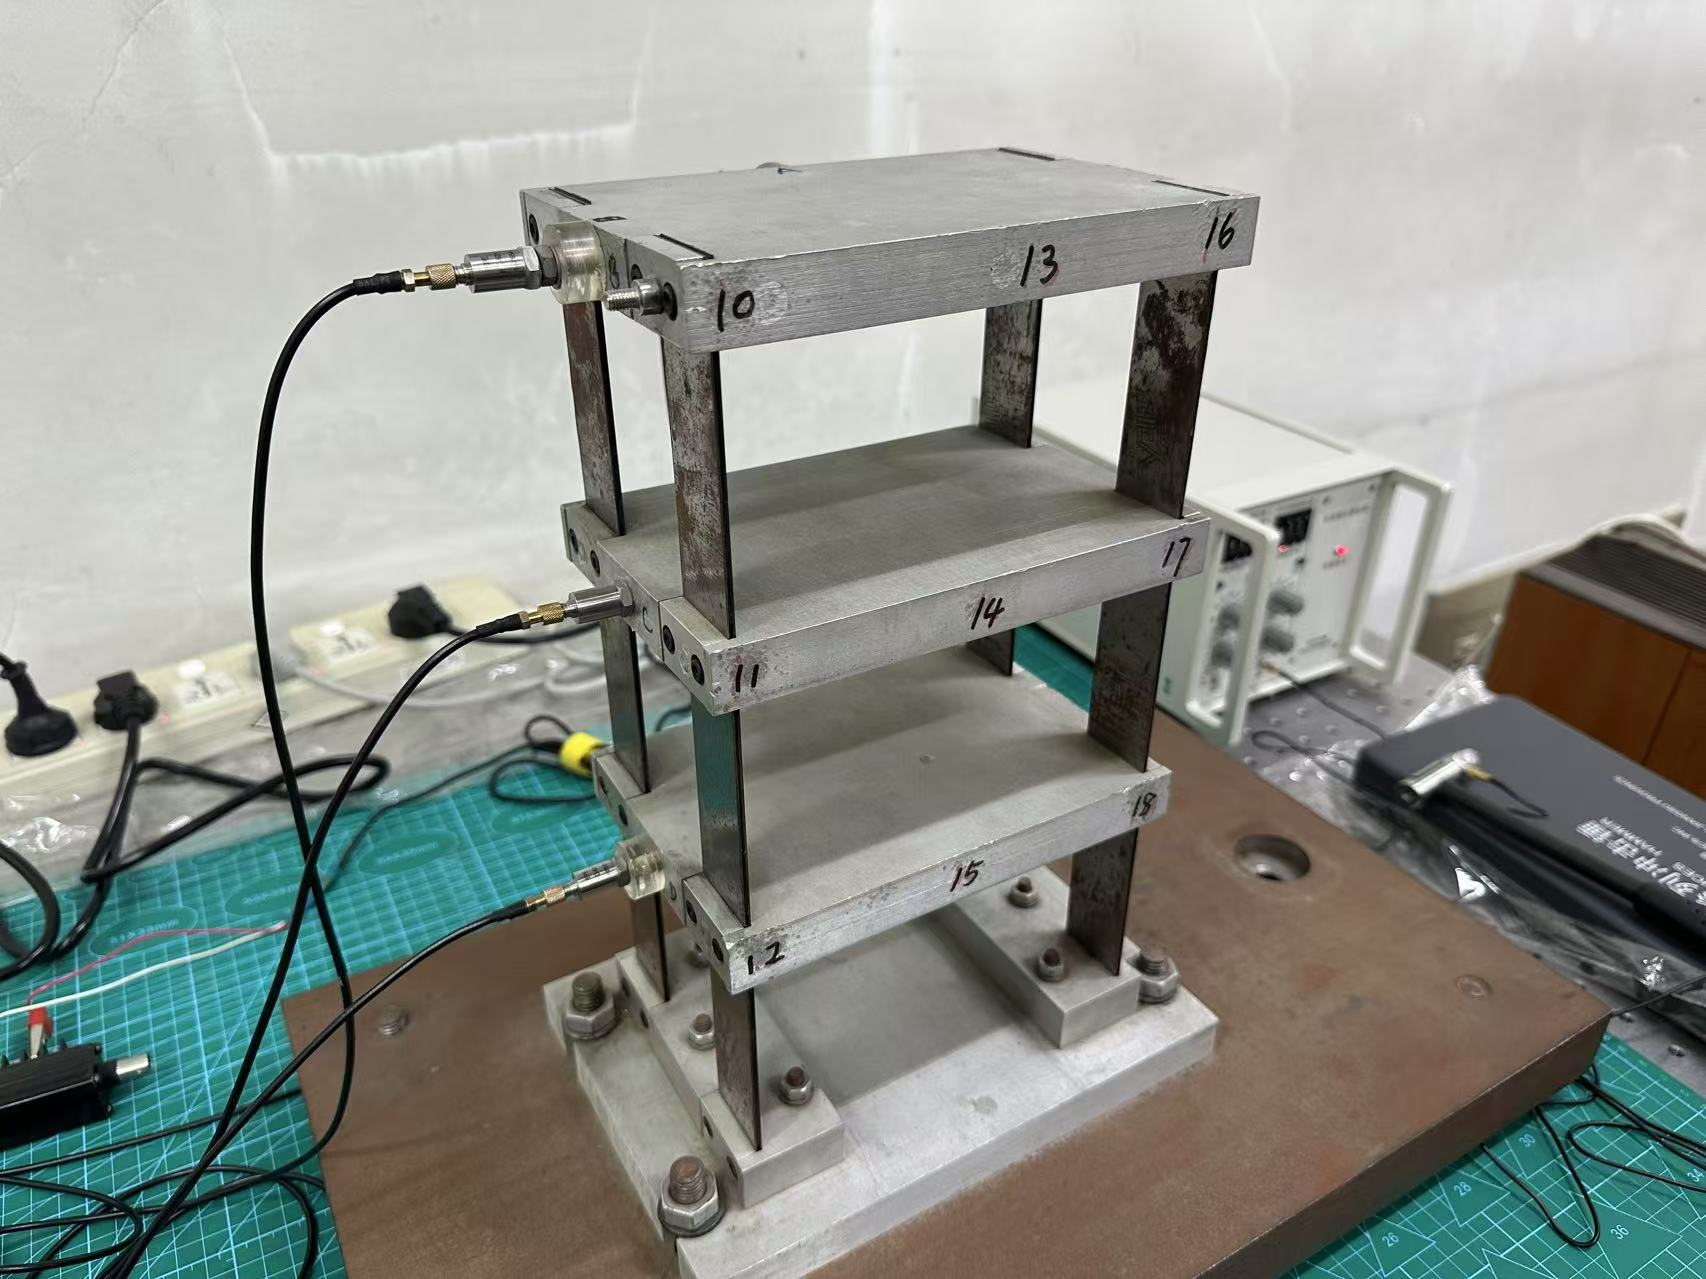
\includegraphics[width=0.52\textwidth]{p03_img01.jpeg}
  \caption{三层楼房模型}
  \label{fig:exp4-model}
\end{figure}

\begin{figure}[H]
  \centering
  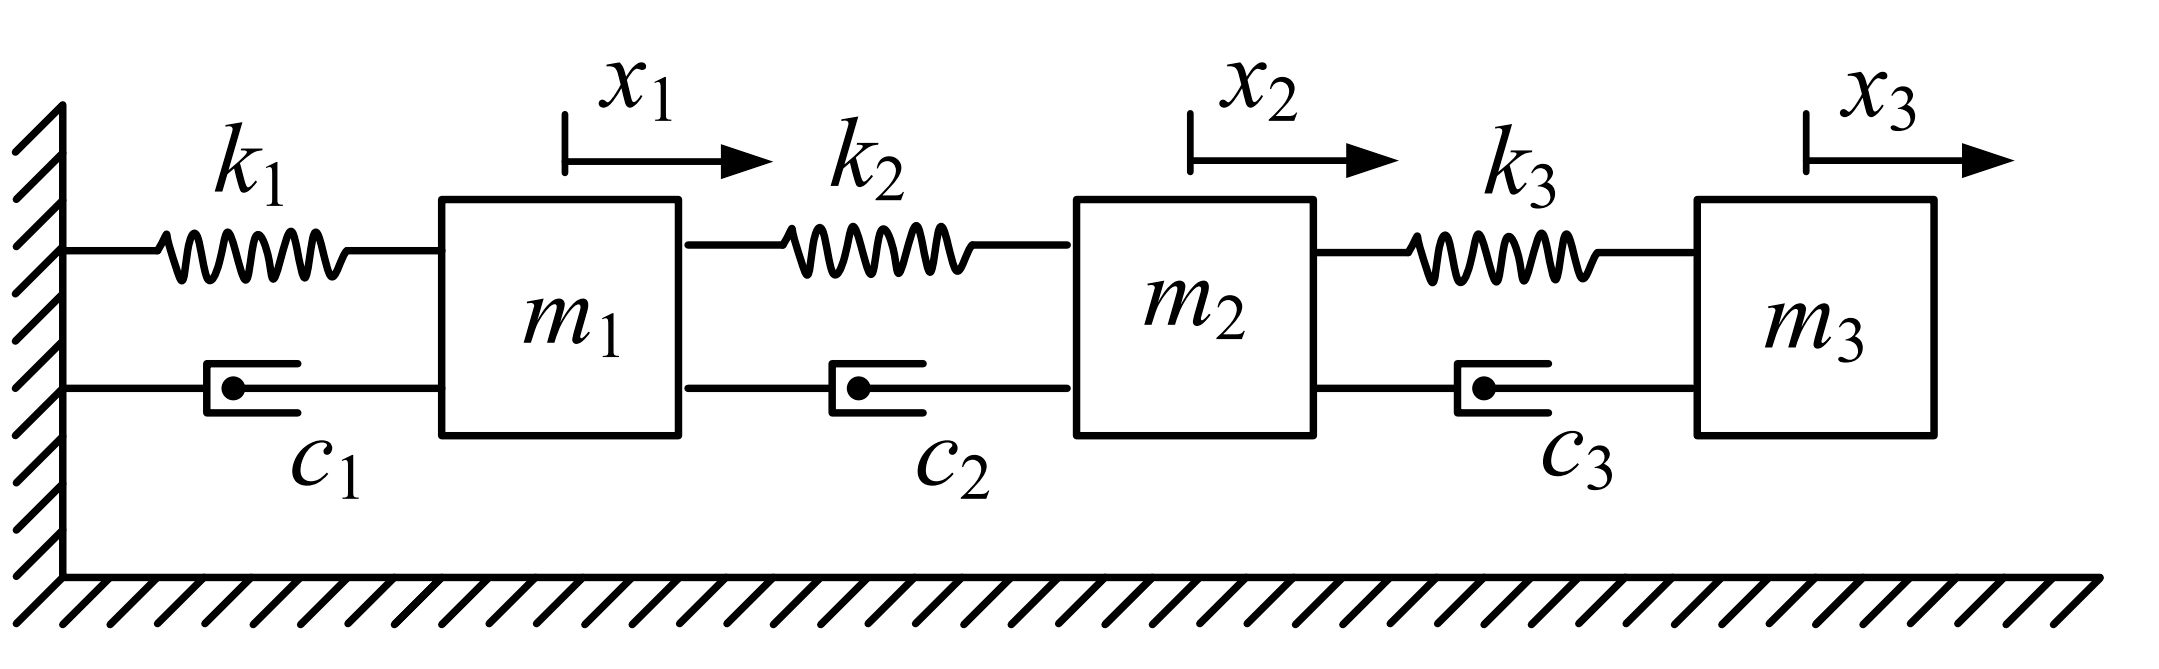
\includegraphics[width=0.56\textwidth]{p03_img02.png}
  \caption{三自由度计算模型}
  \label{fig:exp4-3dof}
\end{figure}

该系统的动力学平衡方程为
\begin{equation}
\begin{aligned}
&\begin{bmatrix}
 m_1&0&0\\0&m_2&0\\0&0&m_3
\end{bmatrix}
\begin{Bmatrix}\ddot{x}_1\\\ddot{x}_2\\\ddot{x}_3\end{Bmatrix}
+\begin{bmatrix}
 c_1+c_2&-c_2&0\\-c_2&c_2+c_3&-c_3\\0&-c_3&c_3
\end{bmatrix}
\begin{Bmatrix}\dot{x}_1\\\dot{x}_2\\\dot{x}_3\end{Bmatrix}\\
&\quad+\begin{bmatrix}
 k_1+k_2&-k_2&0\\-k_2&k_2+k_3&-k_3\\0&-k_3&k_3
\end{bmatrix}
\begin{Bmatrix}x_1\\x_2\\x_3\end{Bmatrix}
=\begin{Bmatrix}f_1(t)\\f_2(t)\\f_3(t)\end{Bmatrix}.
\end{aligned}
\end{equation}
当 $m_1=m_2=m_3=m$，$c_1=c_2=c_3=c_4$，$k_1=k_2=k_3=k_4$ 时，阻尼矩阵 $[c]$ 与刚度矩阵 $[k]$ 成比例，此即比例阻尼的一种典型情况，因而具有实模态振型。

若不考虑阻尼的影响，可根据动力学平衡方程求解无阻尼三自由度系统的特征值问题，进而得到该三自由度系统的固有圆频率：
\begin{equation}
  \omega_1=0.445\sqrt{\frac{k}{m}},\qquad
  \omega_2=1.247\sqrt{\frac{k}{m}},\qquad
  \omega_3=1.802\sqrt{\frac{k}{m}}.
\end{equation}
对应的特征向量为
\begin{equation}
  \{\varphi\}_1=\begin{Bmatrix}1\\1.802\\2.247\end{Bmatrix},\qquad
  \{\varphi\}_2=\begin{Bmatrix}1\\0.445\\-0.802\end{Bmatrix},\qquad
  \{\varphi\}_3=\begin{Bmatrix}1\\-1.247\\0.555\end{Bmatrix}.
\end{equation}
得到的固有振型如图\ref{fig:exp4-theoretical-modes}所示。

\begin{figure}[H]
  \centering
  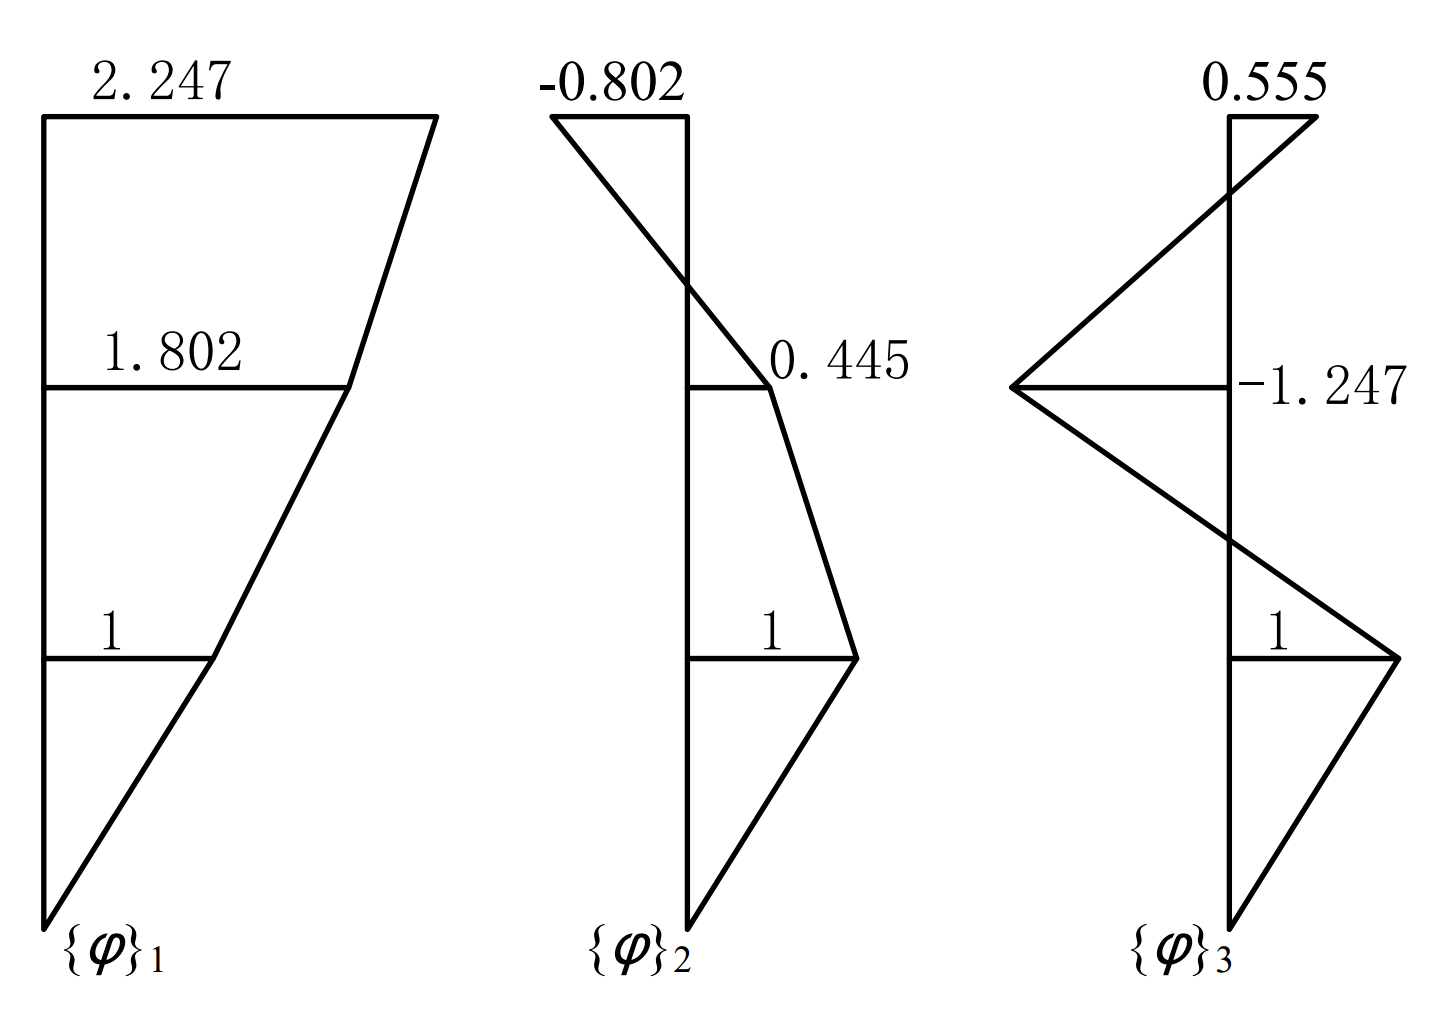
\includegraphics[width=0.36\textwidth]{p04_img01.png}
  \caption{三自由度模型的固有振型}
  \label{fig:exp4-theoretical-modes}
\end{figure}

若需要通过实验测试该模型的频响函数，具体测试实验装置如图\ref{fig:exp4-test-system}所示。针对多自由度系统，若采用单点激励单点接收（SISO）的方法测试，则需要通过多次锤击不同点进行频响函数测量；若采用单点激励多点接收（SIMO）的方法测试，则仅需要一次锤击并多点同时测试，便可进行频响函数测量。

\begin{figure}[H]
  \centering
  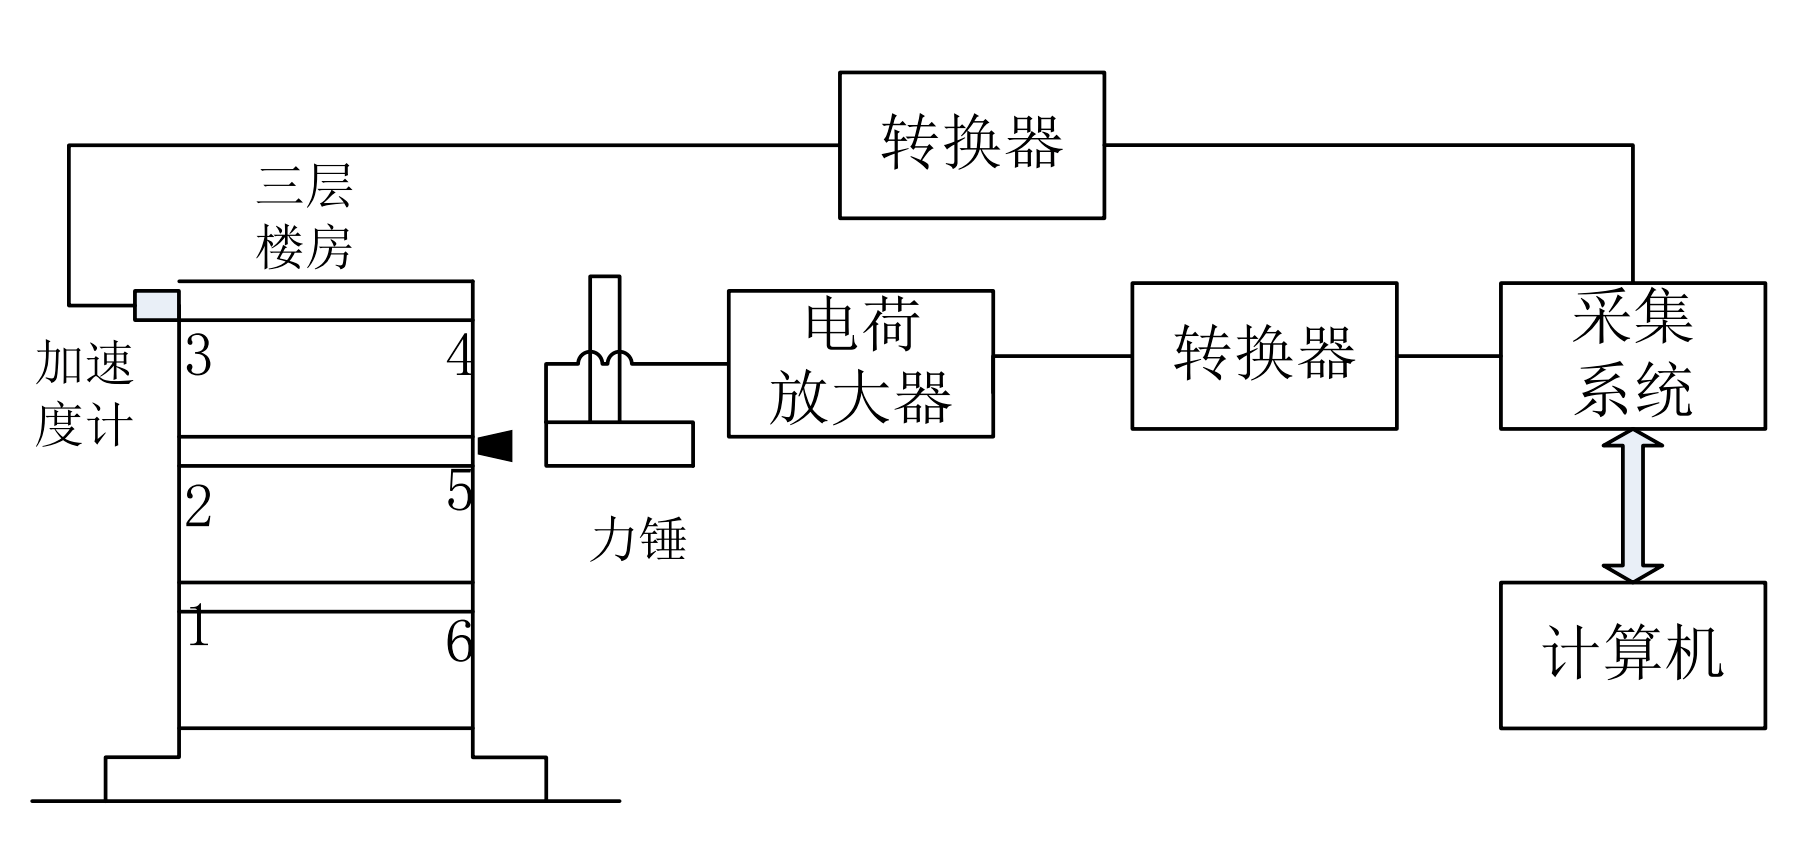
\includegraphics[width=0.48\textwidth]{p04_img02.png}
  \caption{实验装置图}
  \label{fig:exp4-test-system}
\end{figure}

\subsection{实验步骤}
\begin{enumerate}
  \item 在力锤上先装好力传感器，并在三层楼房模型的输出点沿输出方向安装加速度传感器，其轴向灵敏度视型号而定。
  \item 力传感器通过电荷放大器接入动态信号采集系统的 1 通道；加速度传感器经转换器后接入动态信号采集系统的 2--5 通道。
  \item 启动动态信号采集系统软件，先选“路径”，然后在“设置”中进行参数设置。
  \item 测试时先点“保存”选项，再按“采样”进入信号采集等待状态。当锤头以垂直方式敲击楼房模型激励点位置后，等待信号采集完毕并保存数据。重复“采样”和敲击过程，进行 4 组重复性实验。
  \item 最后进行数据浏览，将 1--5 通道的各实验数据导出，进行后续数据处理、频响函数确定和模态参数识别。根据图\ref{fig:exp4-points}标注的各个测试点进行如下实验。
  \item 测试不同锤帽（橡胶、尼龙、钢）力锤敲击的能量频带。力锤分别选用三种锤帽，在模型正面敲击“4”号位置，得到力锤激励信号，并进行 FFT 分析。
  \item 单点敲击（橡胶锤帽）$\Rightarrow$多点响应（SIMO）：在模型正面锤击“4”号位置，经过多次测试，得到另一面 B、C、D 三个点对应采集通道的响应信号。
  \item 多点敲击（橡胶/尼龙锤帽）$\Rightarrow$单点响应（多次 SISO）：
  \begin{enumerate}[label=\alph*)]
    \item 力锤选用橡胶锤帽，在模型正面分别锤击“4”“5”“6”号位置，通过多次测试，在另一面 B 点测得响应信号。
    \item 力锤选用尼龙锤帽，在模型侧面分别锤击“13”“14”“15”号位置，通过多次测试，在另一面 A 点测得响应信号。
  \end{enumerate}
  \item 多点敲击（钢锤帽）$\Rightarrow$单点响应（多次 SISO）：
  \begin{enumerate}[label=\alph*)]
    \item 力锤选用钢锤帽，分别在模型正面锤击“1”“2”“3”“7”“8”“9”号位置，通过多次测试，在模型侧面的 A 点测得响应信号。
    \item 力锤选用钢锤帽，分别在模型侧面锤击“10”“11”“12”“16”“17”“18”号位置，通过多次测试，在模型正面的 B 点测得响应信号。
  \end{enumerate}
\end{enumerate}

\begin{figure}[H]
  \centering
  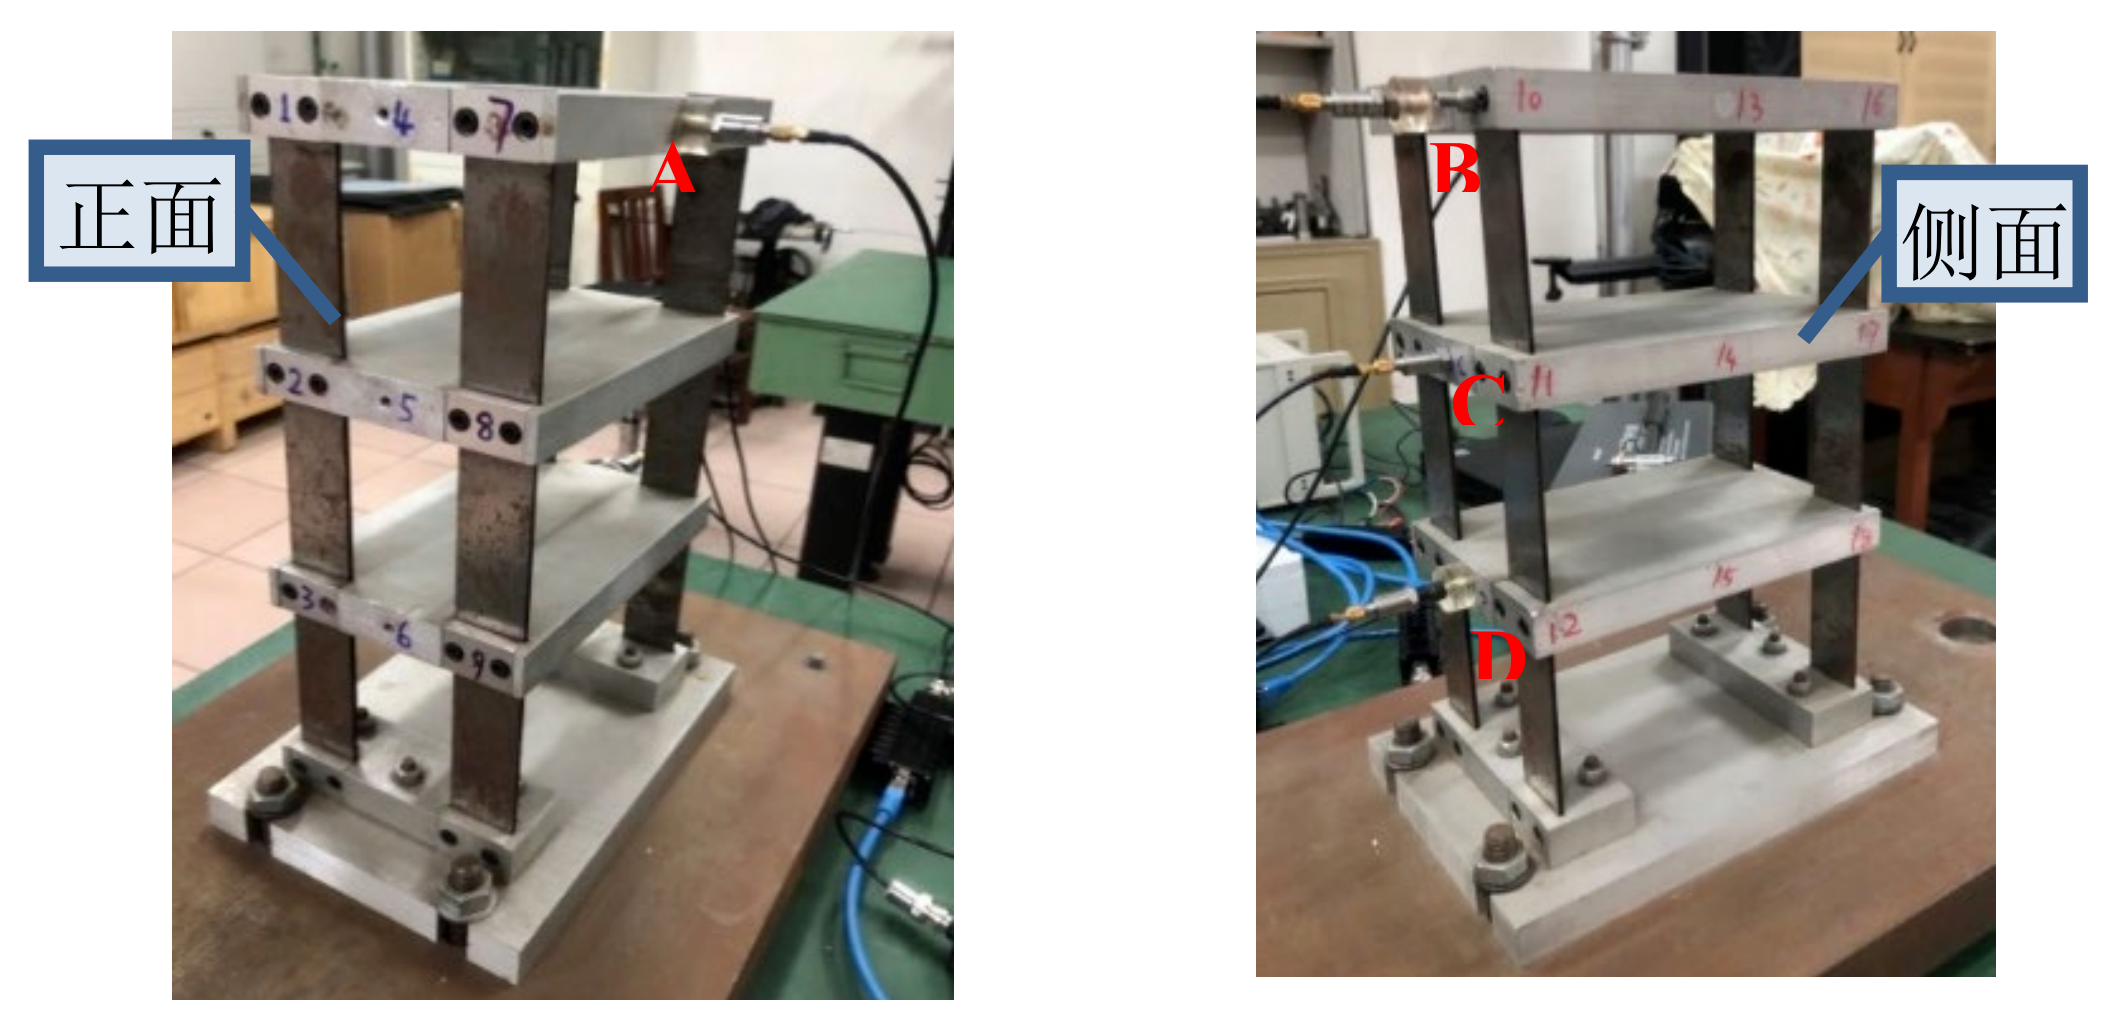
\includegraphics[width=0.5\textwidth]{p05_img01.png}
  \caption{测点的标注位置}
  \label{fig:exp4-points}
\end{figure}

\subsection{实验参数}
请按本组实际设置填写：
\begin{itemize}
  \item 电荷放大器放大倍数：\blank[2.5cm]。
  \item A 通道加速度传感器修正系数：\blank[2.5cm]；B 通道：\blank[2.5cm]。
  \item C 通道加速度传感器修正系数：\blank[2.5cm]；D 通道：\blank[2.5cm]。
  \item 触发选择：内部触发；触发方式：高电平触发；触发通道：力传感器 CH1 通道；触发幅值：\blank[2cm]；提前/滞后：\blank[2cm] 点；采集时长：\blank[2cm]；采样频率：\blank[2cm]。
\end{itemize}

\section{实验测量结果}
\noindent\textbf{使用说明：}以下结果图均从原报告提取，便于保留图件和读图示例。写作时请用同名文件替换为本组曲线或振型图，并填写本组数据。

\subsection{测试不同锤帽（橡胶、尼龙、钢）力锤敲击的能量频带}
分别使用橡胶、尼龙和钢锤帽，在模型正面“4”号位置施加激励。对采集数据进行时域可视化，得到力锤激励信号；随后进行 FFT 分析，并对频域数据进行平均化处理，得到不同锤帽力锤敲击的能量频带，如图\ref{fig:exp4-hammer-band}所示。

\begin{figure}[H]
\centering
\subcaptionbox{橡胶锤帽平均激励信号}[0.47\textwidth]{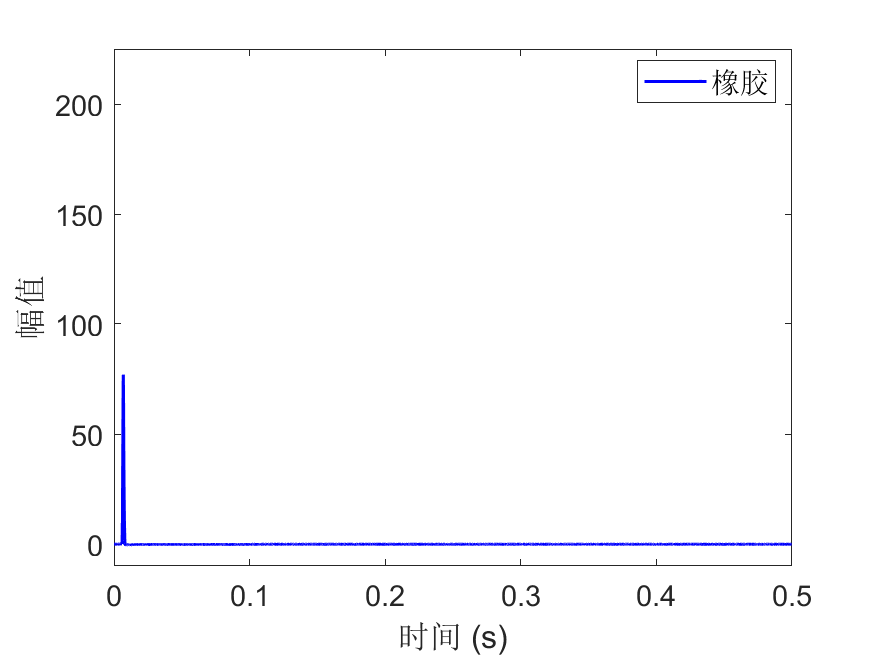
\includegraphics[width=\linewidth]{p06_img01.png}}\hfill
\subcaptionbox{尼龙锤帽平均激励信号}[0.47\textwidth]{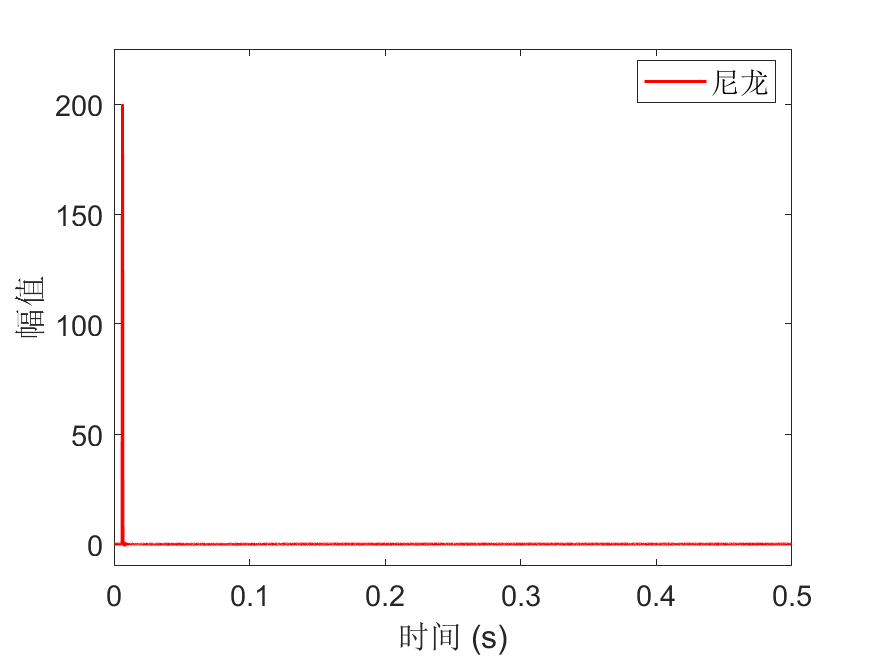
\includegraphics[width=\linewidth]{p06_img02.png}}\\[0.5em]
\subcaptionbox{钢锤帽平均激励信号}[0.47\textwidth]{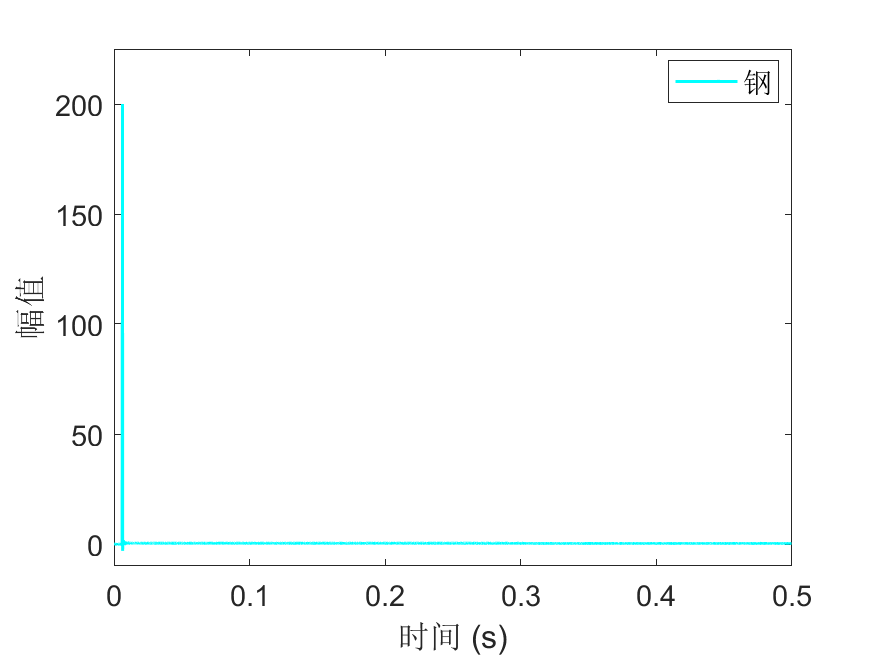
\includegraphics[width=\linewidth]{p06_img03.png}}\hfill
\subcaptionbox{三种锤帽激励平均能量频带}[0.47\textwidth]{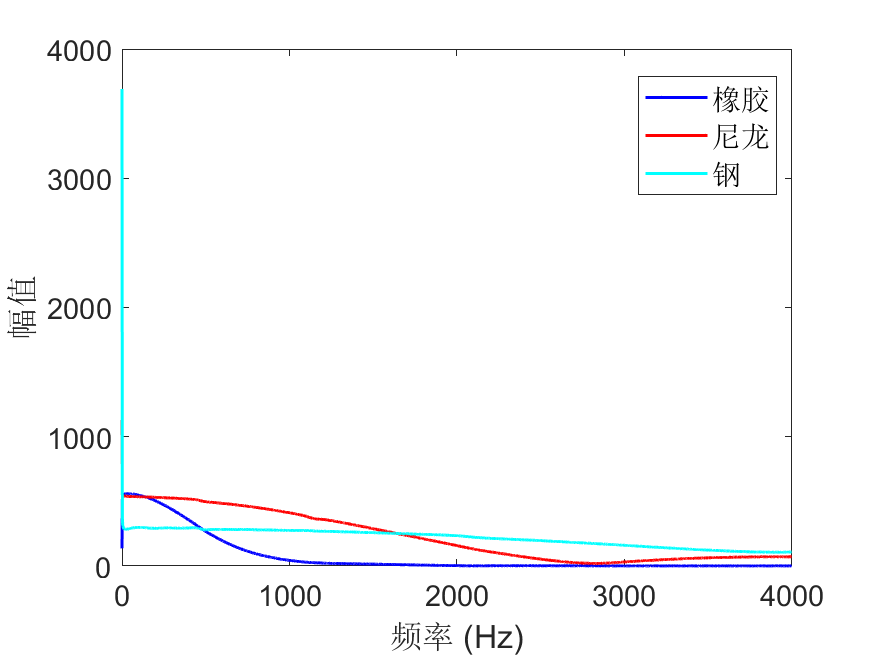
\includegraphics[width=\linewidth]{p06_img04.png}}
\caption{橡胶锤帽、尼龙锤帽、钢锤帽得到的激励信号以及能量频带}
\label{fig:exp4-hammer-band}
\end{figure}

从图中读取并填写：橡胶锤头激励信号带宽约为\blank[2cm] Hz，尼龙锤头激励信号带宽约为\blank[2cm] Hz，钢锤头激励信号带宽约为\blank[2cm] Hz。本实验采样频率为\blank[2cm] Hz。

分析锤帽材料硬度与激励频带宽度的关系，并说明测量低频或高频固有频率结构时应如何选择锤帽。
\answer

\subsection{单点敲击（橡胶锤帽）\texorpdfstring{$\Rightarrow$}{⇒}多点响应（SIMO）}
力锤选用橡胶锤帽，在模型正面“4”号位置进行敲击。经过多次测试，采集另一面 B、C、D 三个点对应的响应信号。通过快速傅里叶变换（FFT）得到平均后的频响函数，如图\ref{fig:exp4-rubber-simo-frf}所示。

\begin{figure}[H]
\centering
\subcaptionbox{平均幅频曲线}[0.47\textwidth]{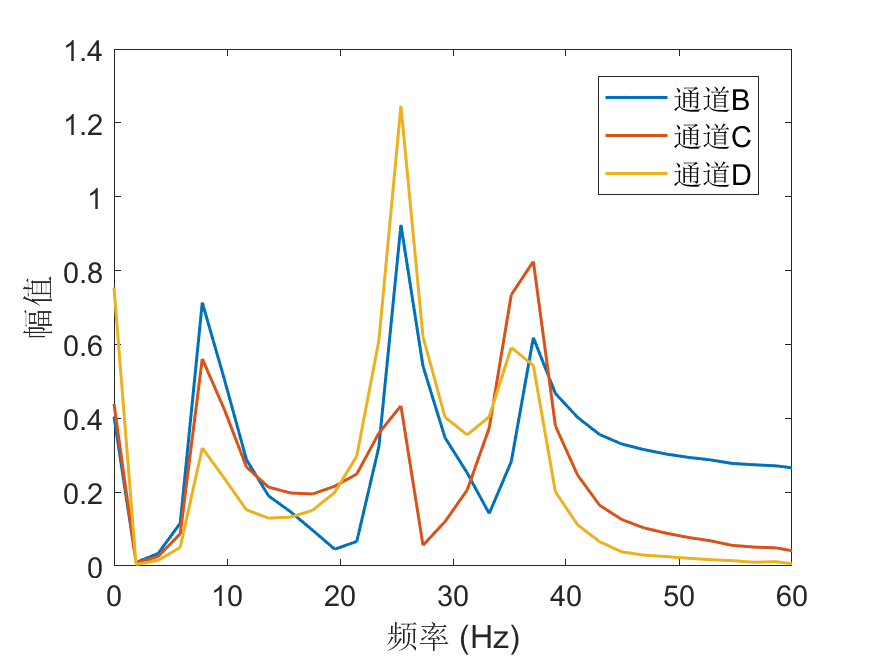
\includegraphics[width=\linewidth]{p07_img01.png}}\hfill
\subcaptionbox{平均实频曲线}[0.47\textwidth]{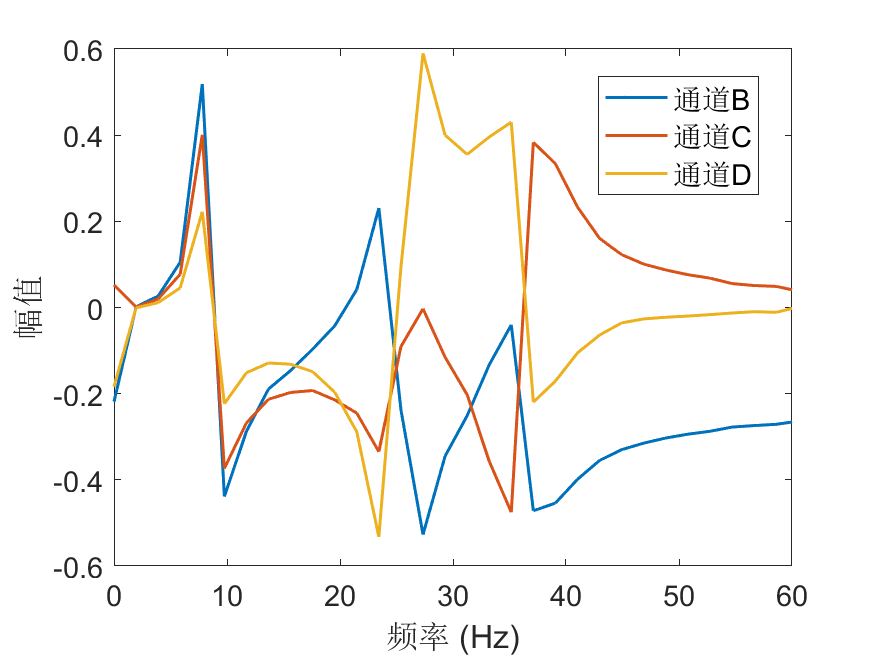
\includegraphics[width=\linewidth]{p07_img02.png}}\\[0.5em]
\subcaptionbox{平均虚频曲线}[0.47\textwidth]{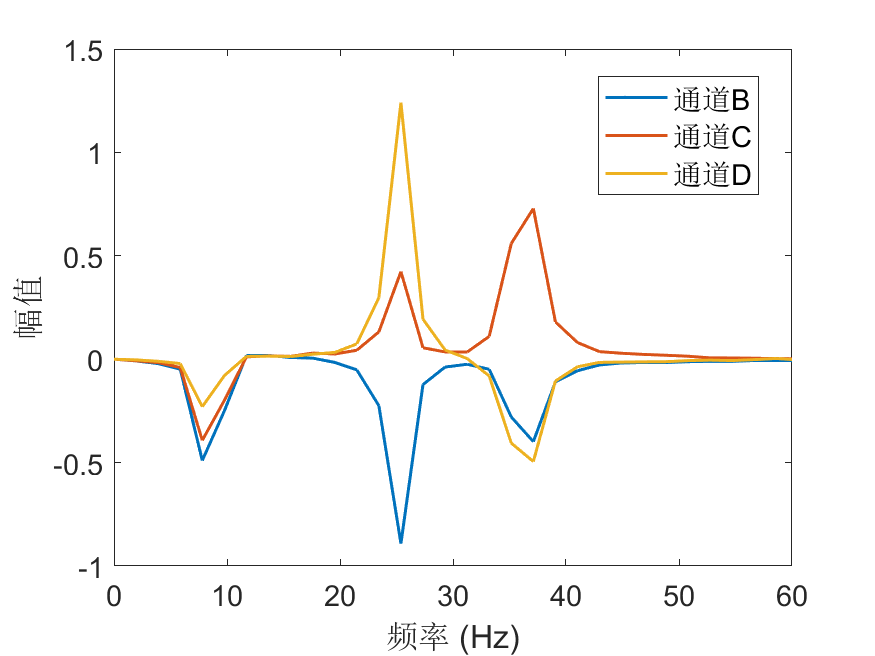
\includegraphics[width=\linewidth]{p07_img03.png}}\hfill
\subcaptionbox{平均相频曲线}[0.47\textwidth]{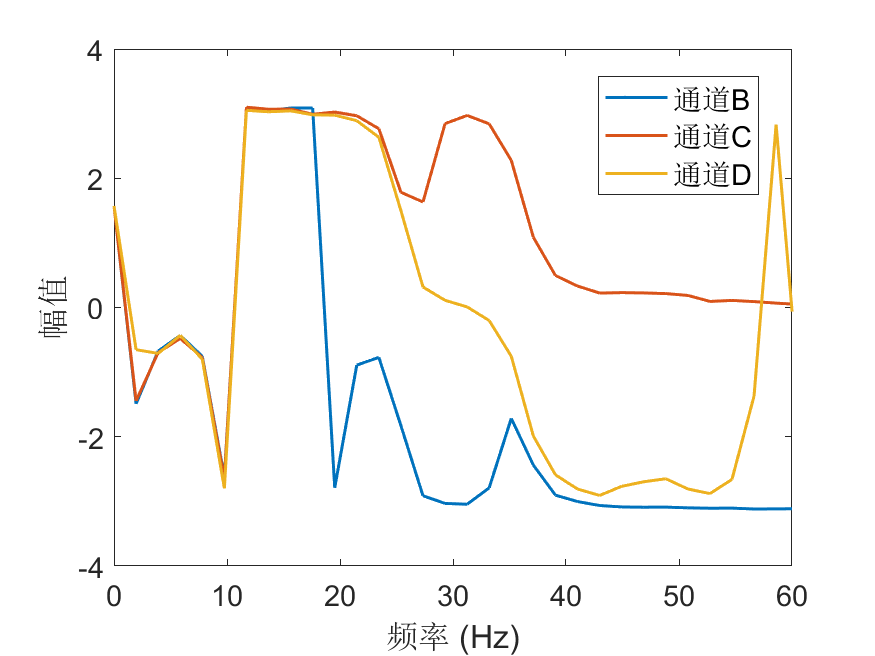
\includegraphics[width=\linewidth]{p07_img04.png}}
\caption{橡胶锤帽正面锤击 SIMO 频响函数曲线}
\label{fig:exp4-rubber-simo-frf}
\end{figure}

本实验使用加速度传感器测量对应点的加速度，因此其对应虚频曲线的幅值相连即为振动模态的振型。将 D 通道信号幅值归一化为 1，绘制成比例的幅值图，如图\ref{fig:exp4-rubber-simo-mode}所示。

\begin{figure}[H]
  \centering
  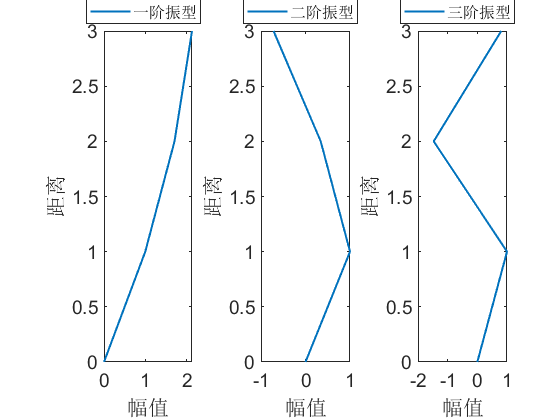
\includegraphics[width=0.5\textwidth]{p08_img01.png}
  \caption{橡胶锤帽正面锤击 SIMO 振型图}
  \label{fig:exp4-rubber-simo-mode}
\end{figure}

对应的振动模态为
\begin{equation}
  \{\varphi\}_1=\begin{Bmatrix}1\\\blank[1.2cm]\\\blank[1.2cm]\end{Bmatrix},\qquad
  \{\varphi\}_2=\begin{Bmatrix}1\\\blank[1.2cm]\\\blank[1.2cm]\end{Bmatrix},\qquad
  \{\varphi\}_3=\begin{Bmatrix}1\\\blank[1.2cm]\\\blank[1.2cm]\end{Bmatrix}.
\end{equation}
实频函数的零点与虚频函数的极值点对应的频率即为结构固有频率。由此获得弯曲振动前三阶固有频率，填入表\ref{tab:exp4-rubber-simo-frequency}。

\begin{table}[H]
\centering
\caption{橡胶锤帽正面锤击 SIMO 前三阶固有频率}
\label{tab:exp4-rubber-simo-frequency}
\begin{tabular}{lccc}
\toprule
阶数 & 一阶 & 二阶 & 三阶\\
\midrule
通道 B（Hz） & \blank[1.8cm] & \blank[1.8cm] & \blank[1.8cm]\\
通道 C（Hz） & \blank[1.8cm] & \blank[1.8cm] & \blank[1.8cm]\\
通道 D（Hz） & \blank[1.8cm] & \blank[1.8cm] & \blank[1.8cm]\\
平均（Hz） & \blank[1.8cm] & \blank[1.8cm] & \blank[1.8cm]\\
\bottomrule
\end{tabular}
\end{table}

阻尼比可通过实频曲线波峰和波谷对应的频率计算。设 $\omega_a$ 与 $\omega_b$ 分别为实频曲线波峰与波谷对应的频率，$\omega_0$ 为虚频曲线波峰或波谷对应的频率，则
\begin{equation}
  \zeta=\frac{\omega_b-\omega_a}{2\omega_0}.
  \label{eq:exp4-damping}
\end{equation}
各阶模态阻尼比填入表\ref{tab:exp4-rubber-simo-damping}。

\begin{table}[H]
\centering
\caption{橡胶锤帽正面锤击 SIMO 阻尼比}
\label{tab:exp4-rubber-simo-damping}
\begin{tabular}{lccc}
\toprule
阶数 & 一阶 & 二阶 & 三阶\\
\midrule
通道 B & \blank[1.8cm] & \blank[1.8cm] & \blank[1.8cm]\\
通道 C & \blank[1.8cm] & \blank[1.8cm] & \blank[1.8cm]\\
通道 D & \blank[1.8cm] & \blank[1.8cm] & \blank[1.8cm]\\
平均 & \blank[1.8cm] & \blank[1.8cm] & \blank[1.8cm]\\
\bottomrule
\end{tabular}
\end{table}

\subsection{多点敲击（橡胶/尼龙锤帽）\texorpdfstring{$\Rightarrow$}{⇒}单点响应（多次 SISO）}
\subsubsection{橡胶锤帽正面锤击}
力锤选用橡胶锤帽，在模型正面分别锤击“4”“5”“6”号位置，通过多次测试，在另一面 B 点测得响应信号。通过 FFT 得到平均后的频响函数，如图\ref{fig:exp4-rubber-siso-frf}所示。

\begin{figure}[H]
\centering
\subcaptionbox{平均幅频曲线}[0.47\textwidth]{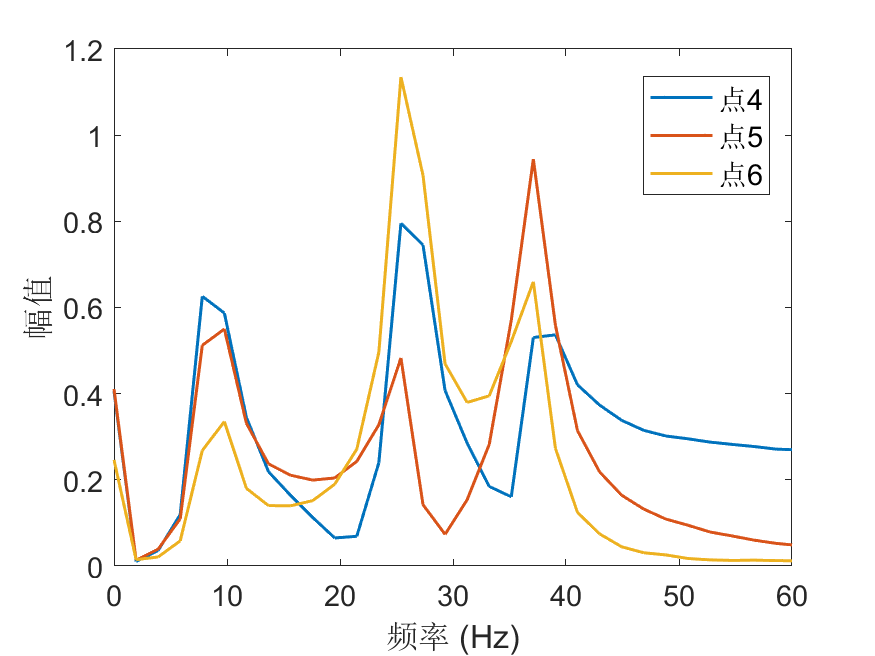
\includegraphics[width=\linewidth]{p09_img01.png}}\hfill
\subcaptionbox{平均实频曲线}[0.47\textwidth]{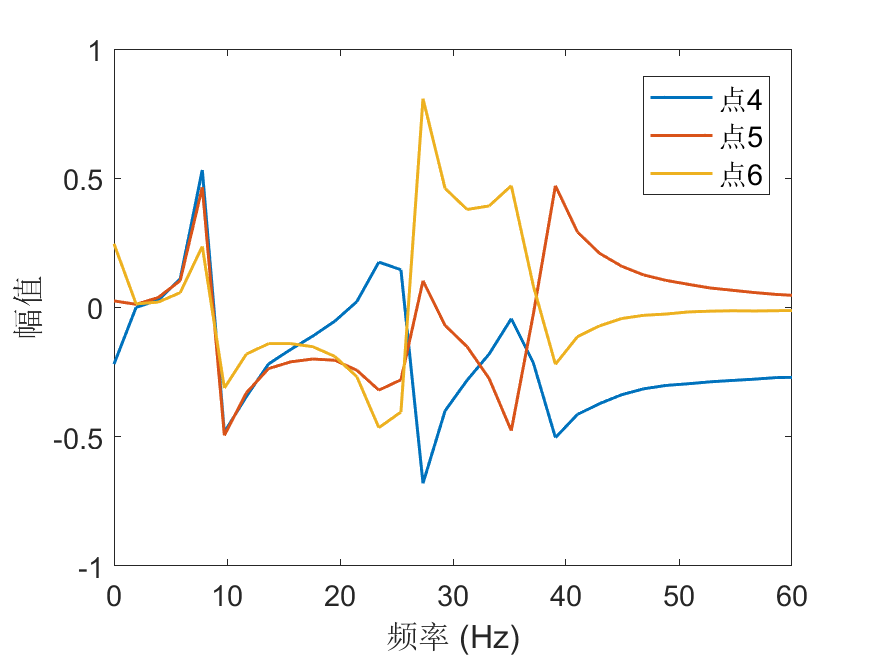
\includegraphics[width=\linewidth]{p09_img02.png}}\\[0.5em]
\subcaptionbox{平均虚频曲线}[0.47\textwidth]{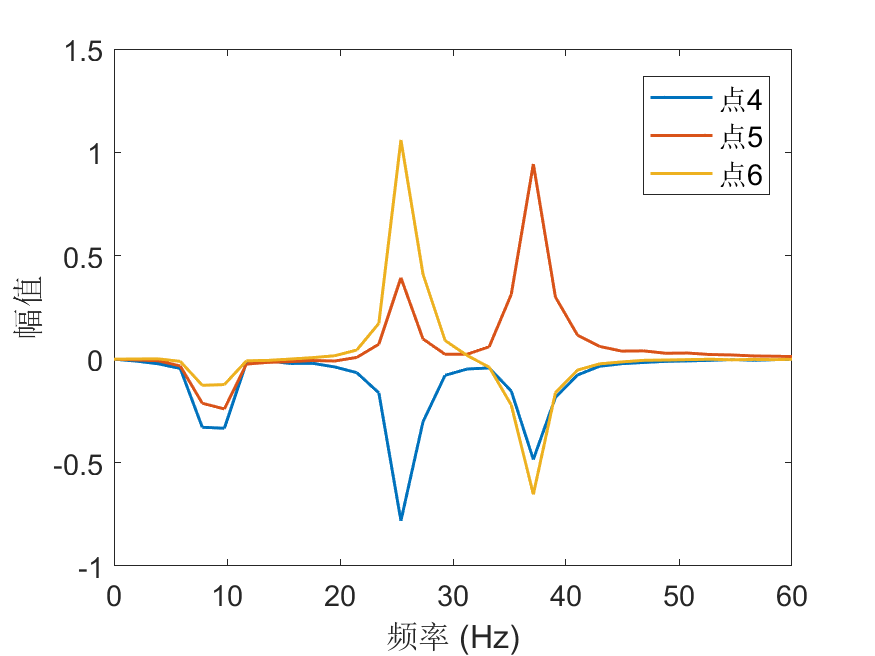
\includegraphics[width=\linewidth]{p09_img03.png}}\hfill
\subcaptionbox{平均相频曲线}[0.47\textwidth]{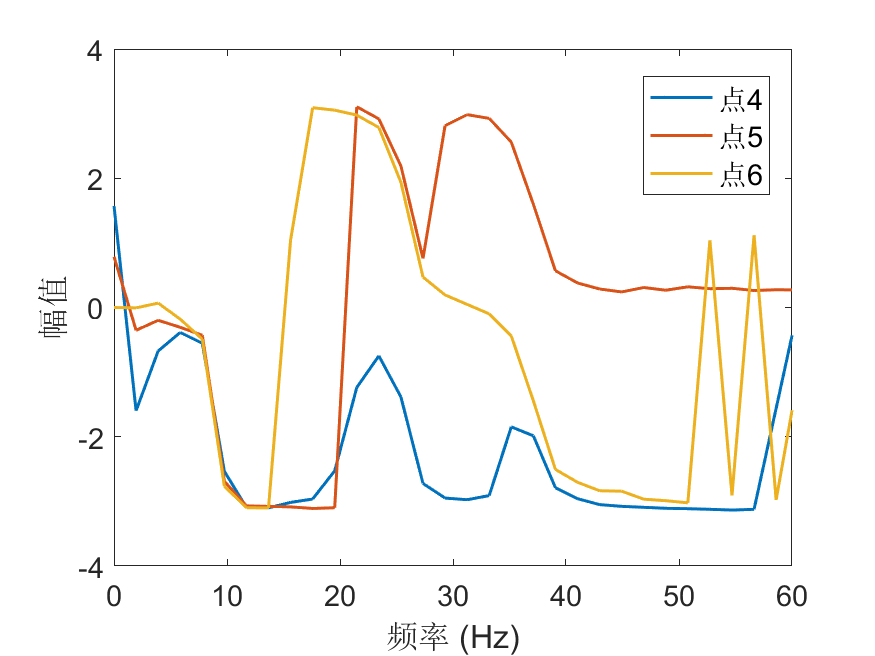
\includegraphics[width=\linewidth]{p09_img04.png}}
\caption{橡胶锤帽正面锤击 SISO 频响函数曲线}
\label{fig:exp4-rubber-siso-frf}
\end{figure}

将点 4 对应的幅值归一化为 1，绘制成比例的幅值图，如图\ref{fig:exp4-rubber-siso-mode}所示。

\begin{figure}[H]
  \centering
  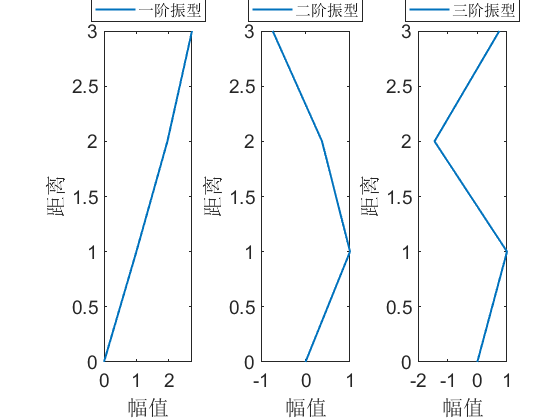
\includegraphics[width=0.5\textwidth]{p09_img05.png}
  \caption{橡胶锤帽正面锤击 SISO 振型图}
  \label{fig:exp4-rubber-siso-mode}
\end{figure}

对应的振动模态为
\begin{equation}
  \{\varphi\}_1=\begin{Bmatrix}1\\\blank[1.2cm]\\\blank[1.2cm]\end{Bmatrix},\qquad
  \{\varphi\}_2=\begin{Bmatrix}1\\\blank[1.2cm]\\\blank[1.2cm]\end{Bmatrix},\qquad
  \{\varphi\}_3=\begin{Bmatrix}1\\\blank[1.2cm]\\\blank[1.2cm]\end{Bmatrix}.
\end{equation}
实频函数零点和虚频函数极值点对应固有频率，据此得到弯曲振动前三阶固有频率，填入表\ref{tab:exp4-rubber-siso-frequency}。按式\eqref{eq:exp4-damping}计算阻尼比，填入表\ref{tab:exp4-rubber-siso-damping}。

\begin{table}[H]
\centering
\caption{橡胶锤帽正面锤击 SISO 前三阶固有频率}
\label{tab:exp4-rubber-siso-frequency}
\begin{tabular}{lccc}
\toprule
阶数 & 一阶 & 二阶 & 三阶\\
\midrule
锤击4点（Hz） & \blank[1.8cm] & \blank[1.8cm] & \blank[1.8cm]\\
锤击5点（Hz） & \blank[1.8cm] & \blank[1.8cm] & \blank[1.8cm]\\
锤击6点（Hz） & \blank[1.8cm] & \blank[1.8cm] & \blank[1.8cm]\\
平均（Hz） & \blank[1.8cm] & \blank[1.8cm] & \blank[1.8cm]\\
\bottomrule
\end{tabular}
\end{table}

\begin{table}[H]
\centering
\caption{橡胶锤帽正面锤击 SISO 阻尼比}
\label{tab:exp4-rubber-siso-damping}
\begin{tabular}{lccc}
\toprule
阶数 & 一阶 & 二阶 & 三阶\\
\midrule
锤击4点 & \blank[1.8cm] & \blank[1.8cm] & \blank[1.8cm]\\
锤击5点 & \blank[1.8cm] & \blank[1.8cm] & \blank[1.8cm]\\
锤击6点 & \blank[1.8cm] & \blank[1.8cm] & \blank[1.8cm]\\
平均 & \blank[1.8cm] & \blank[1.8cm] & \blank[1.8cm]\\
\bottomrule
\end{tabular}
\end{table}

\subsubsection{尼龙锤帽侧面锤击}
力锤选用尼龙锤帽，在模型侧面分别锤击“13”“14”“15”号位置，通过多次测试，在另一面 A 点测得响应信号。通过 FFT 得到平均后的频响函数，如图\ref{fig:exp4-nylon-siso-frf}所示。

\begin{figure}[H]
\centering
\subcaptionbox{平均幅频曲线}[0.47\textwidth]{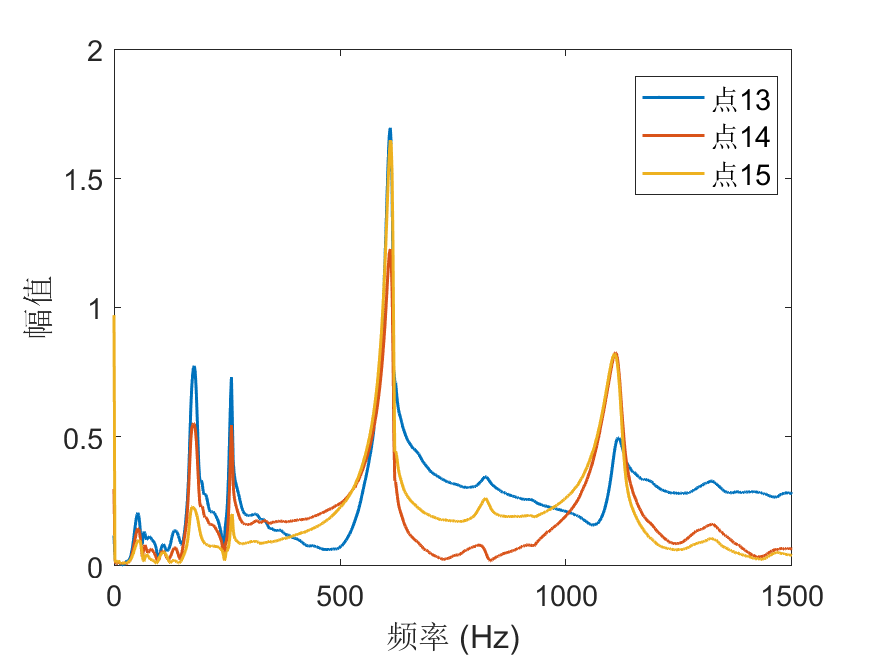
\includegraphics[width=\linewidth]{p11_img01.png}}\hfill
\subcaptionbox{平均实频曲线}[0.47\textwidth]{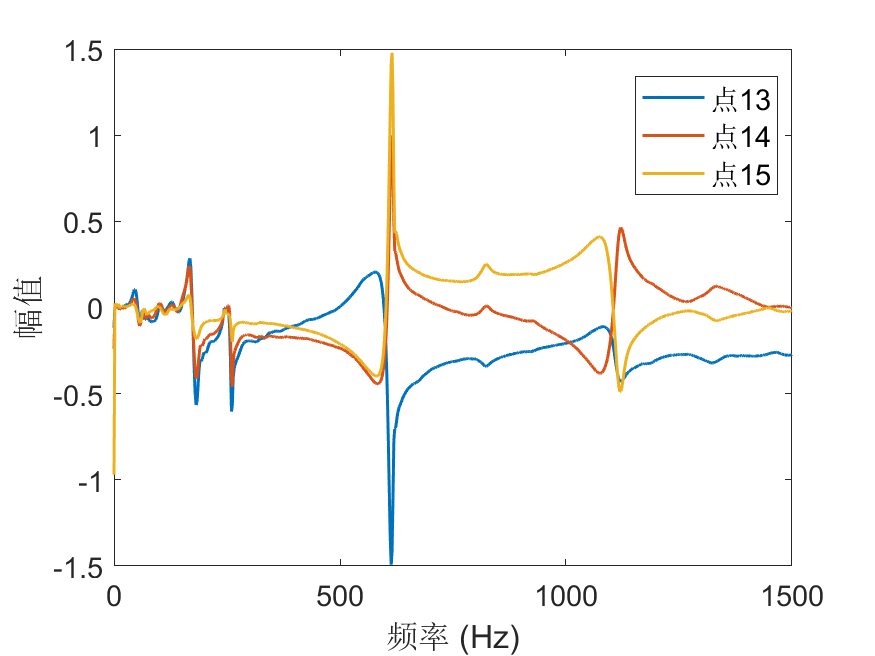
\includegraphics[width=\linewidth]{p11_img02.png}}\\[0.5em]
\subcaptionbox{平均虚频曲线}[0.47\textwidth]{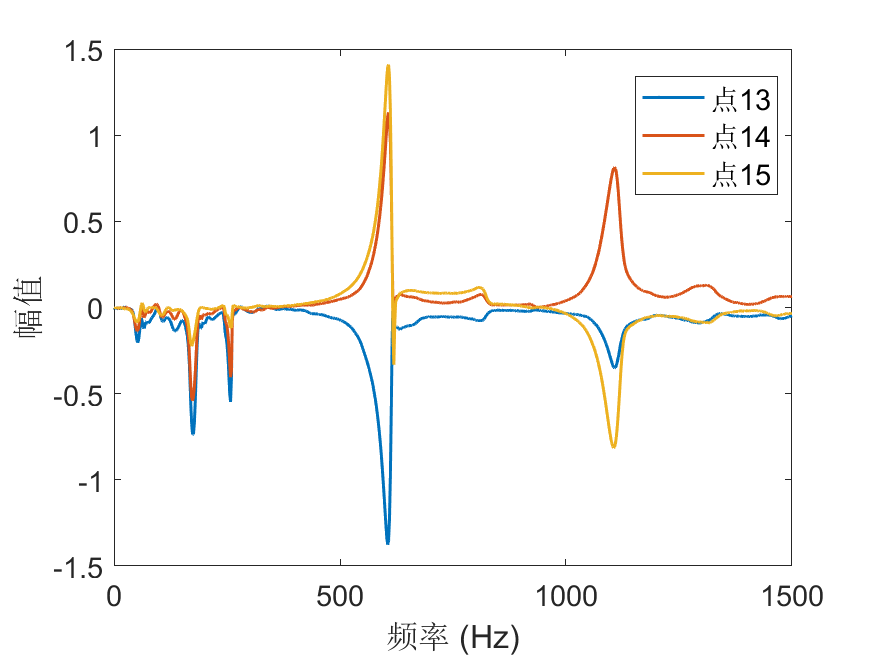
\includegraphics[width=\linewidth]{p11_img03.png}}\hfill
\subcaptionbox{平均相频曲线}[0.47\textwidth]{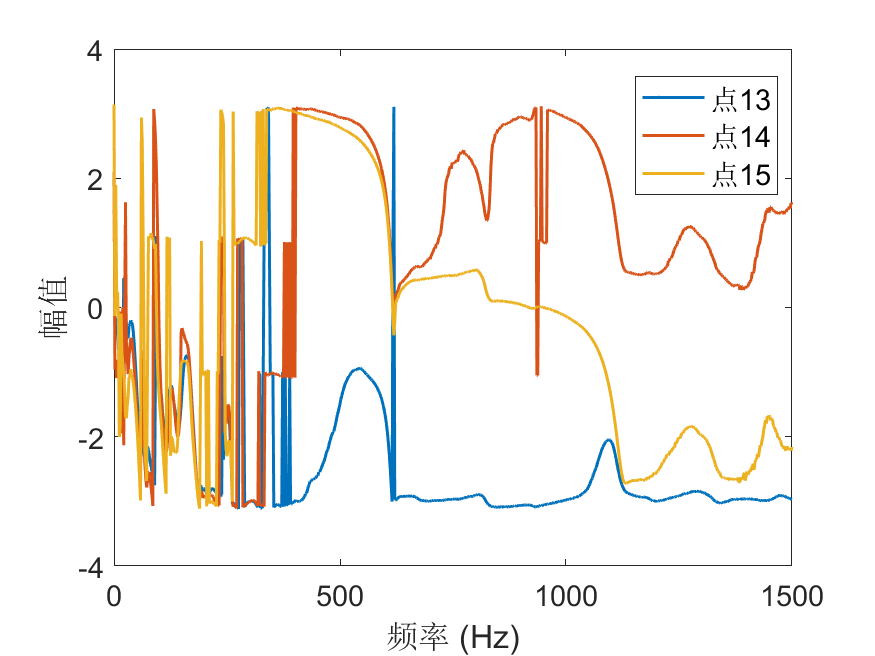
\includegraphics[width=\linewidth]{p11_img04.png}}
\caption{尼龙锤帽侧面锤击 SISO 频响函数曲线}
\label{fig:exp4-nylon-siso-frf}
\end{figure}

将点 15 对应的幅值归一化为 1，绘制成比例的幅值图，如图\ref{fig:exp4-nylon-siso-mode}所示。

\begin{figure}[H]
  \centering
  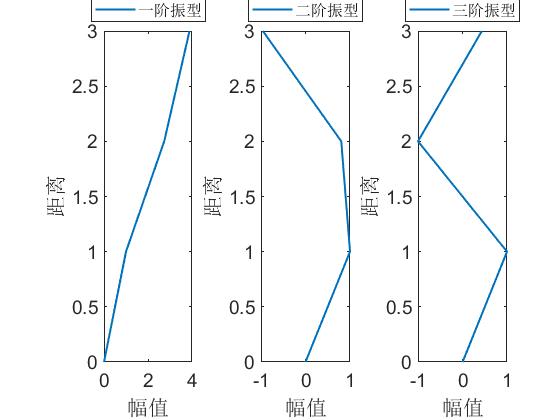
\includegraphics[width=0.5\textwidth]{p11_img05.png}
  \caption{尼龙锤帽侧面锤击 SISO 振型图}
  \label{fig:exp4-nylon-siso-mode}
\end{figure}

对应的振动模态为
\begin{equation}
  \{\varphi\}_1=\begin{Bmatrix}1\\\blank[1.2cm]\\\blank[1.2cm]\end{Bmatrix},\qquad
  \{\varphi\}_2=\begin{Bmatrix}1\\\blank[1.2cm]\\\blank[1.2cm]\end{Bmatrix},\qquad
  \{\varphi\}_3=\begin{Bmatrix}1\\\blank[1.2cm]\\\blank[1.2cm]\end{Bmatrix}.
\end{equation}
前三阶固有频率填入表\ref{tab:exp4-nylon-frequency}，阻尼比填入表\ref{tab:exp4-nylon-damping}。

\begin{table}[H]
\centering
\caption{尼龙锤帽侧面锤击 SISO 前三阶固有频率}
\label{tab:exp4-nylon-frequency}
\begin{tabular}{lccc}
\toprule
阶数 & 一阶 & 二阶 & 三阶\\
\midrule
锤击13点（Hz） & \blank[1.6cm] & \blank[1.6cm] & \blank[1.6cm]\\
锤击14点（Hz） & \blank[1.6cm] & \blank[1.6cm] & \blank[1.6cm]\\
锤击15点（Hz） & \blank[1.6cm] & \blank[1.6cm] & \blank[1.6cm]\\
平均（Hz） & \blank[1.6cm] & \blank[1.6cm] & \blank[1.6cm]\\
\bottomrule
\end{tabular}
\end{table}

\begin{table}[H]
\centering
\caption{尼龙锤帽侧面锤击 SISO 阻尼比}
\label{tab:exp4-nylon-damping}
\begin{tabular}{lccc}
\toprule
阶数 & 一阶 & 二阶 & 三阶\\
\midrule
锤击13点 & \blank[1.8cm] & \blank[1.8cm] & \blank[1.8cm]\\
锤击14点 & \blank[1.8cm] & \blank[1.8cm] & \blank[1.8cm]\\
锤击15点 & \blank[1.8cm] & \blank[1.8cm] & \blank[1.8cm]\\
平均 & \blank[1.8cm] & \blank[1.8cm] & \blank[1.8cm]\\
\bottomrule
\end{tabular}
\end{table}

\subsection{多点敲击（钢锤帽）\texorpdfstring{$\Rightarrow$}{⇒}单点响应（多次 SISO）}
\subsubsection{钢锤帽正面锤击}
力锤选用钢锤帽，分别在模型正面锤击“1”“2”“3”“7”“8”“9”号位置，通过多次测试，在模型侧面的 A 点测得响应信号。通过 FFT 得到平均后的频响函数，如图\ref{fig:exp4-steel-front-frf1}和图\ref{fig:exp4-steel-front-frf2}所示。

\begin{figure}[H]
\centering
\subcaptionbox{平均幅频曲线}[0.47\textwidth]{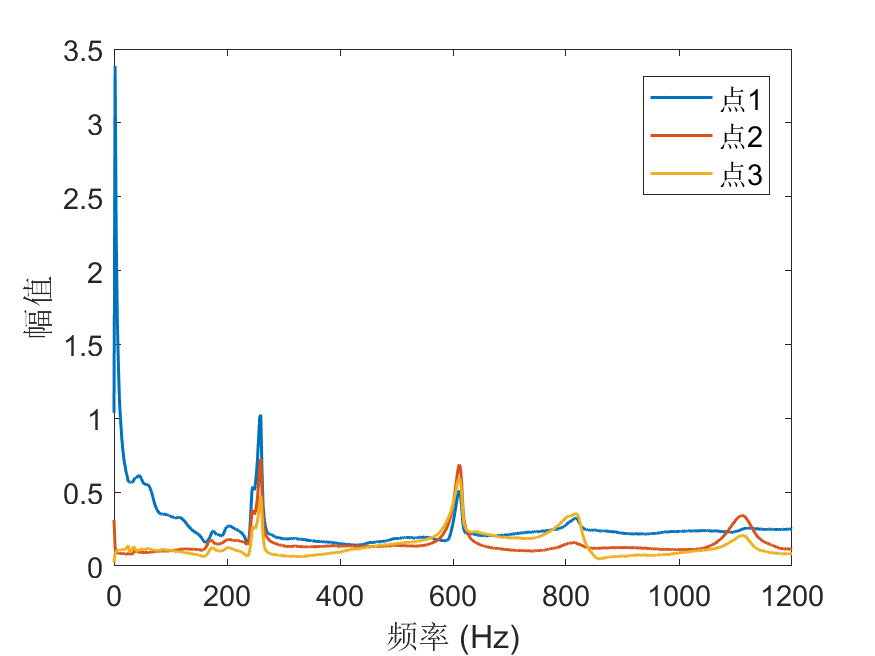
\includegraphics[width=\linewidth]{p12_img01.png}}\hfill
\subcaptionbox{平均实频曲线}[0.47\textwidth]{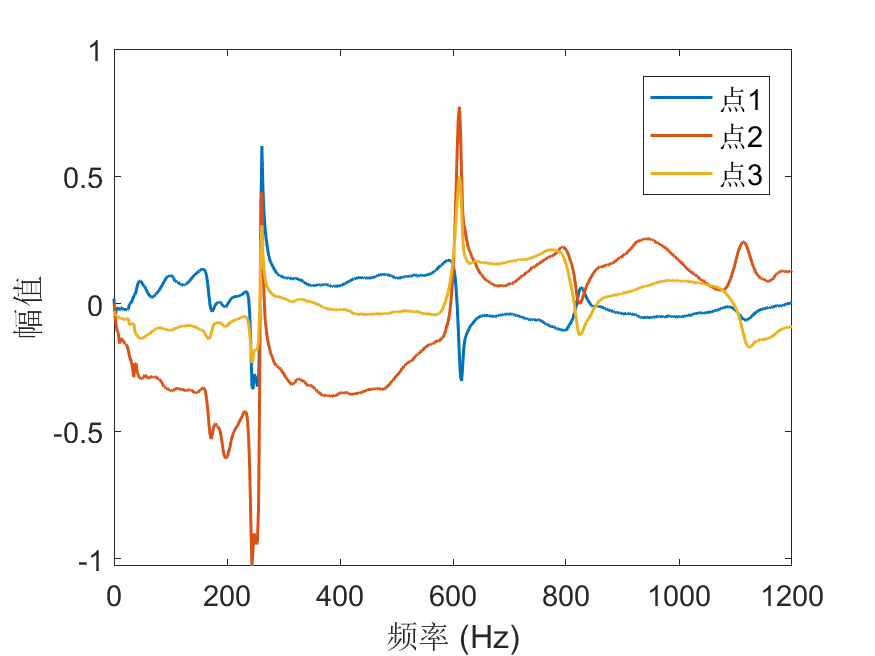
\includegraphics[width=\linewidth]{p12_img02.png}}\\[0.5em]
\subcaptionbox{平均虚频曲线}[0.47\textwidth]{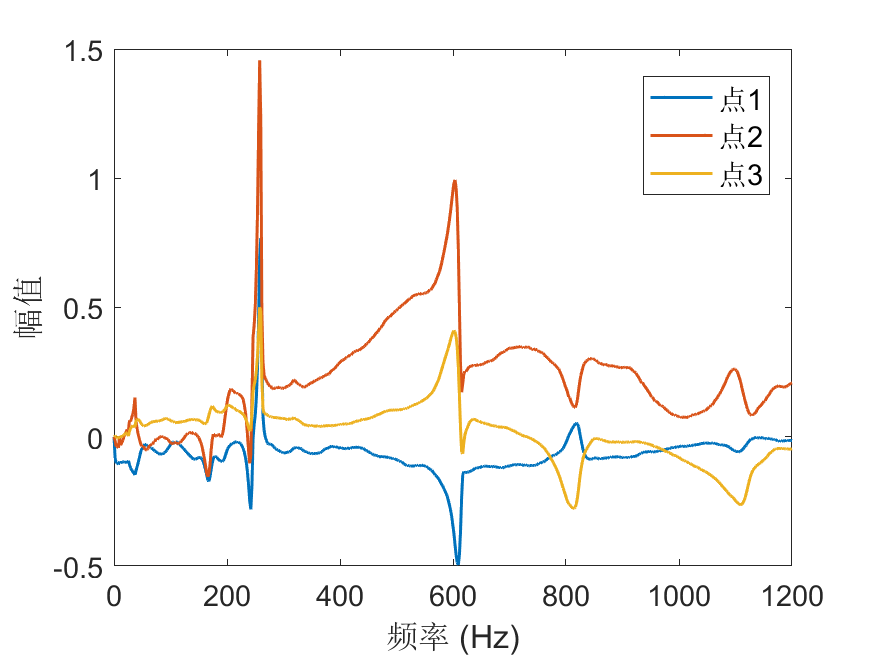
\includegraphics[width=\linewidth]{p12_img03.png}}\hfill
\subcaptionbox{平均相频曲线}[0.47\textwidth]{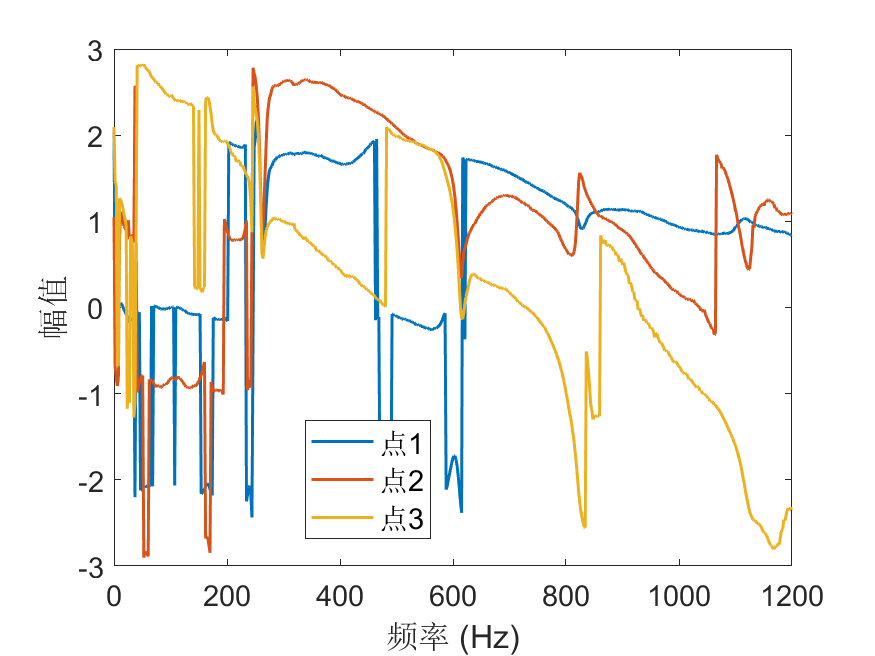
\includegraphics[width=\linewidth]{p12_img04.png}}
\caption{钢锤帽正面锤击 SISO 频响函数曲线（点1、2、3）}
\label{fig:exp4-steel-front-frf1}
\end{figure}

\begin{figure}[H]
\centering
\subcaptionbox{平均幅频曲线}[0.47\textwidth]{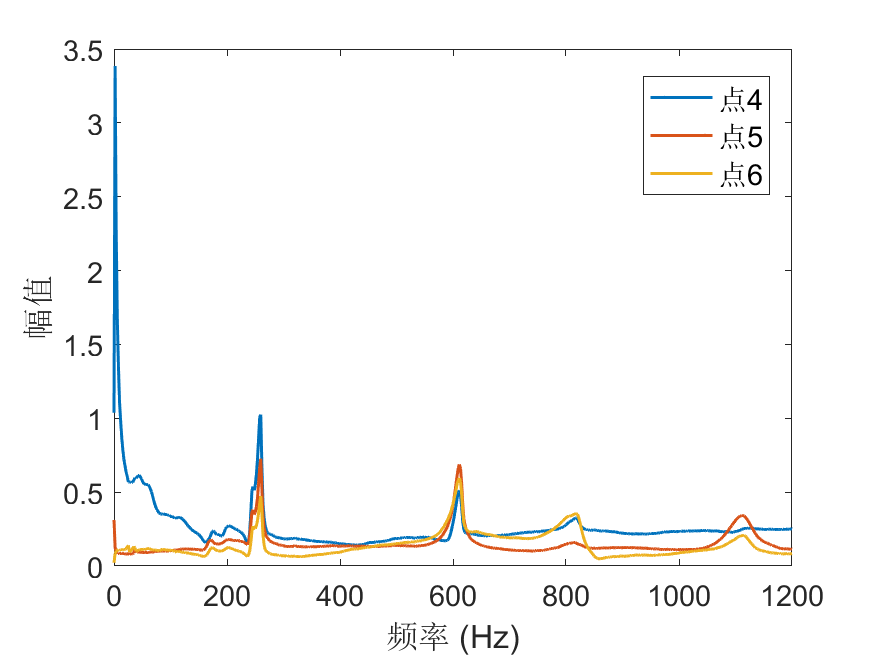
\includegraphics[width=\linewidth]{p13_img01.png}}\hfill
\subcaptionbox{平均实频曲线}[0.47\textwidth]{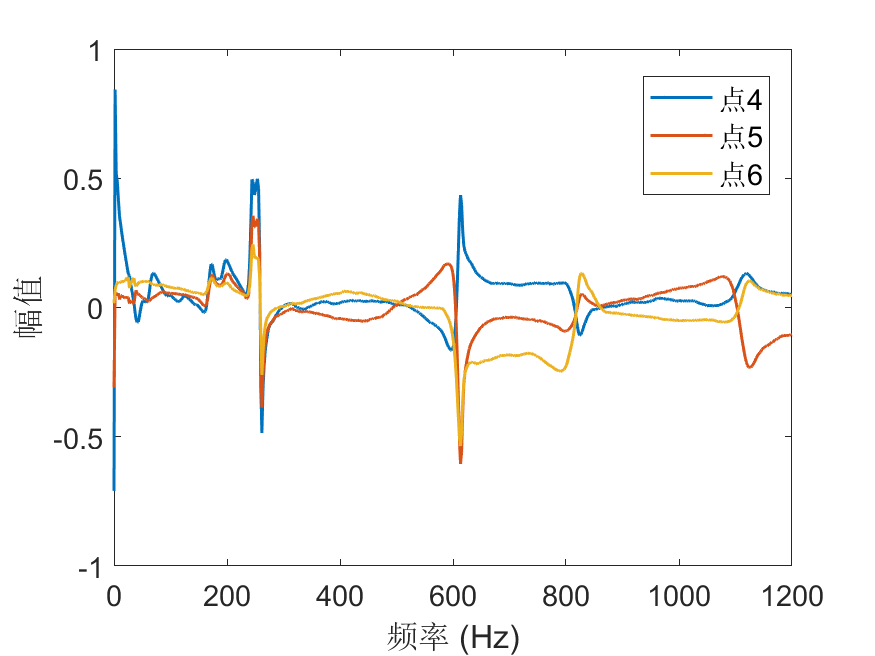
\includegraphics[width=\linewidth]{p13_img02.png}}\\[0.5em]
\subcaptionbox{平均虚频曲线}[0.47\textwidth]{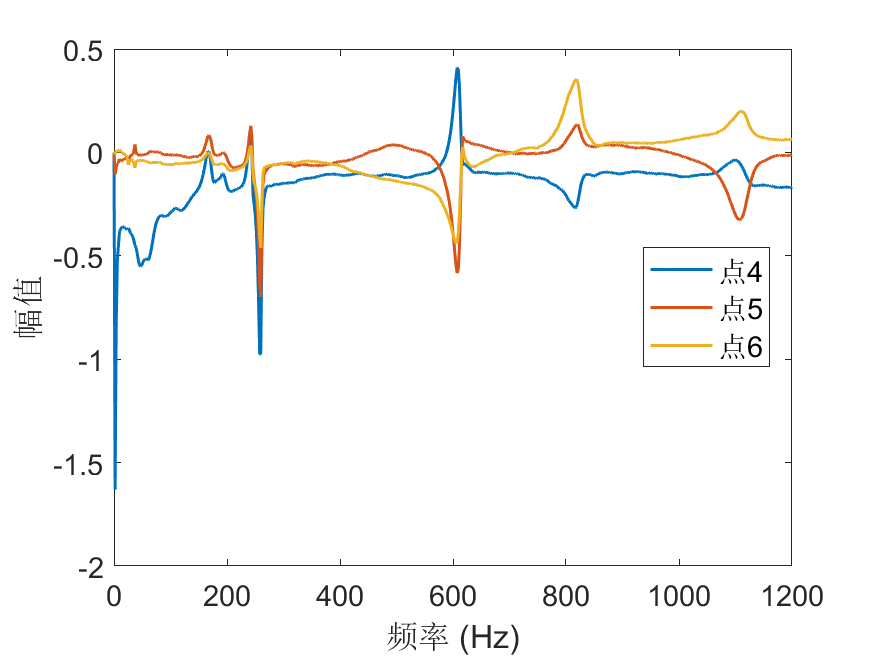
\includegraphics[width=\linewidth]{p13_img03.png}}\hfill
\subcaptionbox{平均相频曲线}[0.47\textwidth]{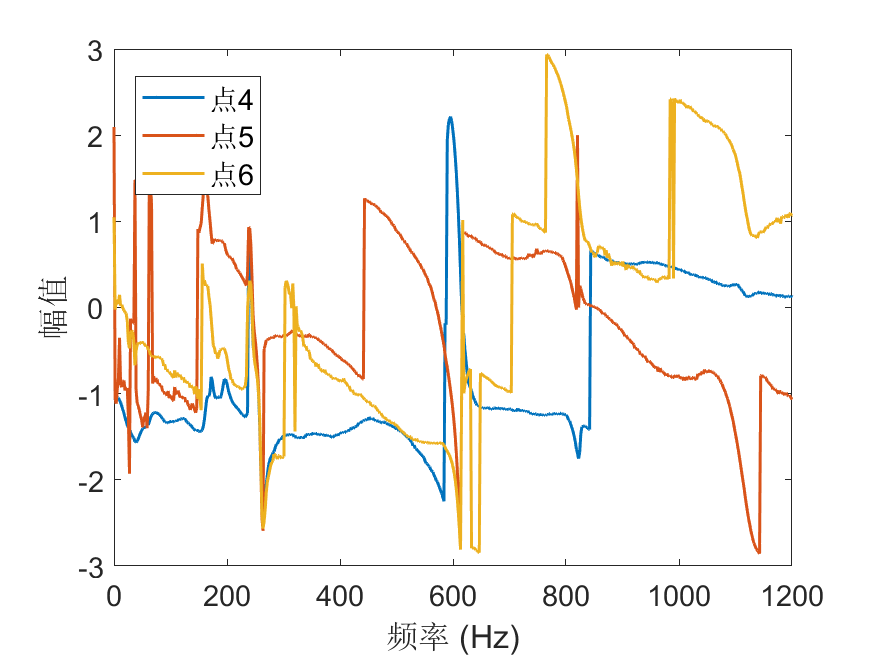
\includegraphics[width=\linewidth]{p13_img04.png}}
\caption{钢锤帽正面锤击 SISO 频响函数曲线（点4、5、6）}
\label{fig:exp4-steel-front-frf2}
\end{figure}

将点 3 与点 9 对应的幅值归一化为 1，绘制成比例的幅值图。图\ref{fig:exp4-steel-front-mode2d}为位于同一竖直线上的点构成的模态图，图\ref{fig:exp4-steel-front-mode3d}为完整三维模态图。

\begin{figure}[H]
\centering
\subcaptionbox{点1、2、3}[0.47\textwidth]{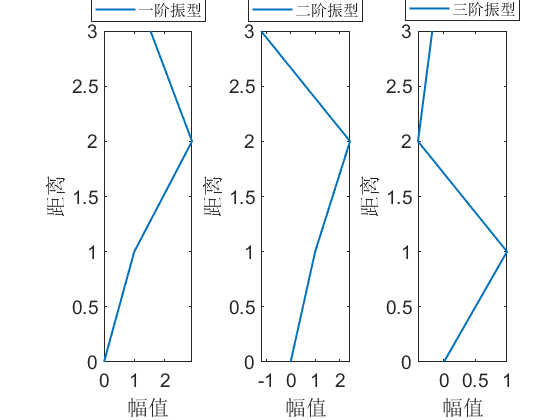
\includegraphics[width=\linewidth]{p13_img05.png}}\hfill
\subcaptionbox{点4、5、6}[0.47\textwidth]{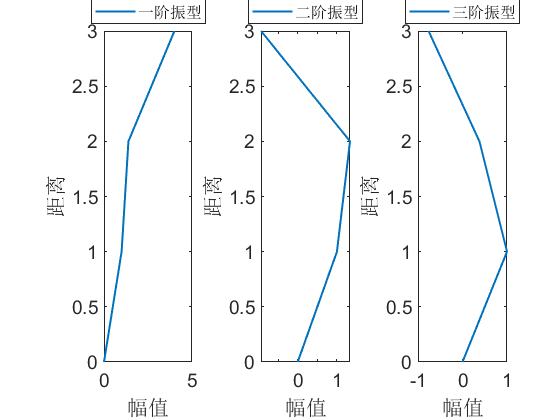
\includegraphics[width=\linewidth]{p13_img06.png}}
\caption{钢锤帽正面锤击 SISO 振型图}
\label{fig:exp4-steel-front-mode2d}
\end{figure}

\begin{figure}[H]
\centering
\subcaptionbox{一阶模态}[0.31\textwidth]{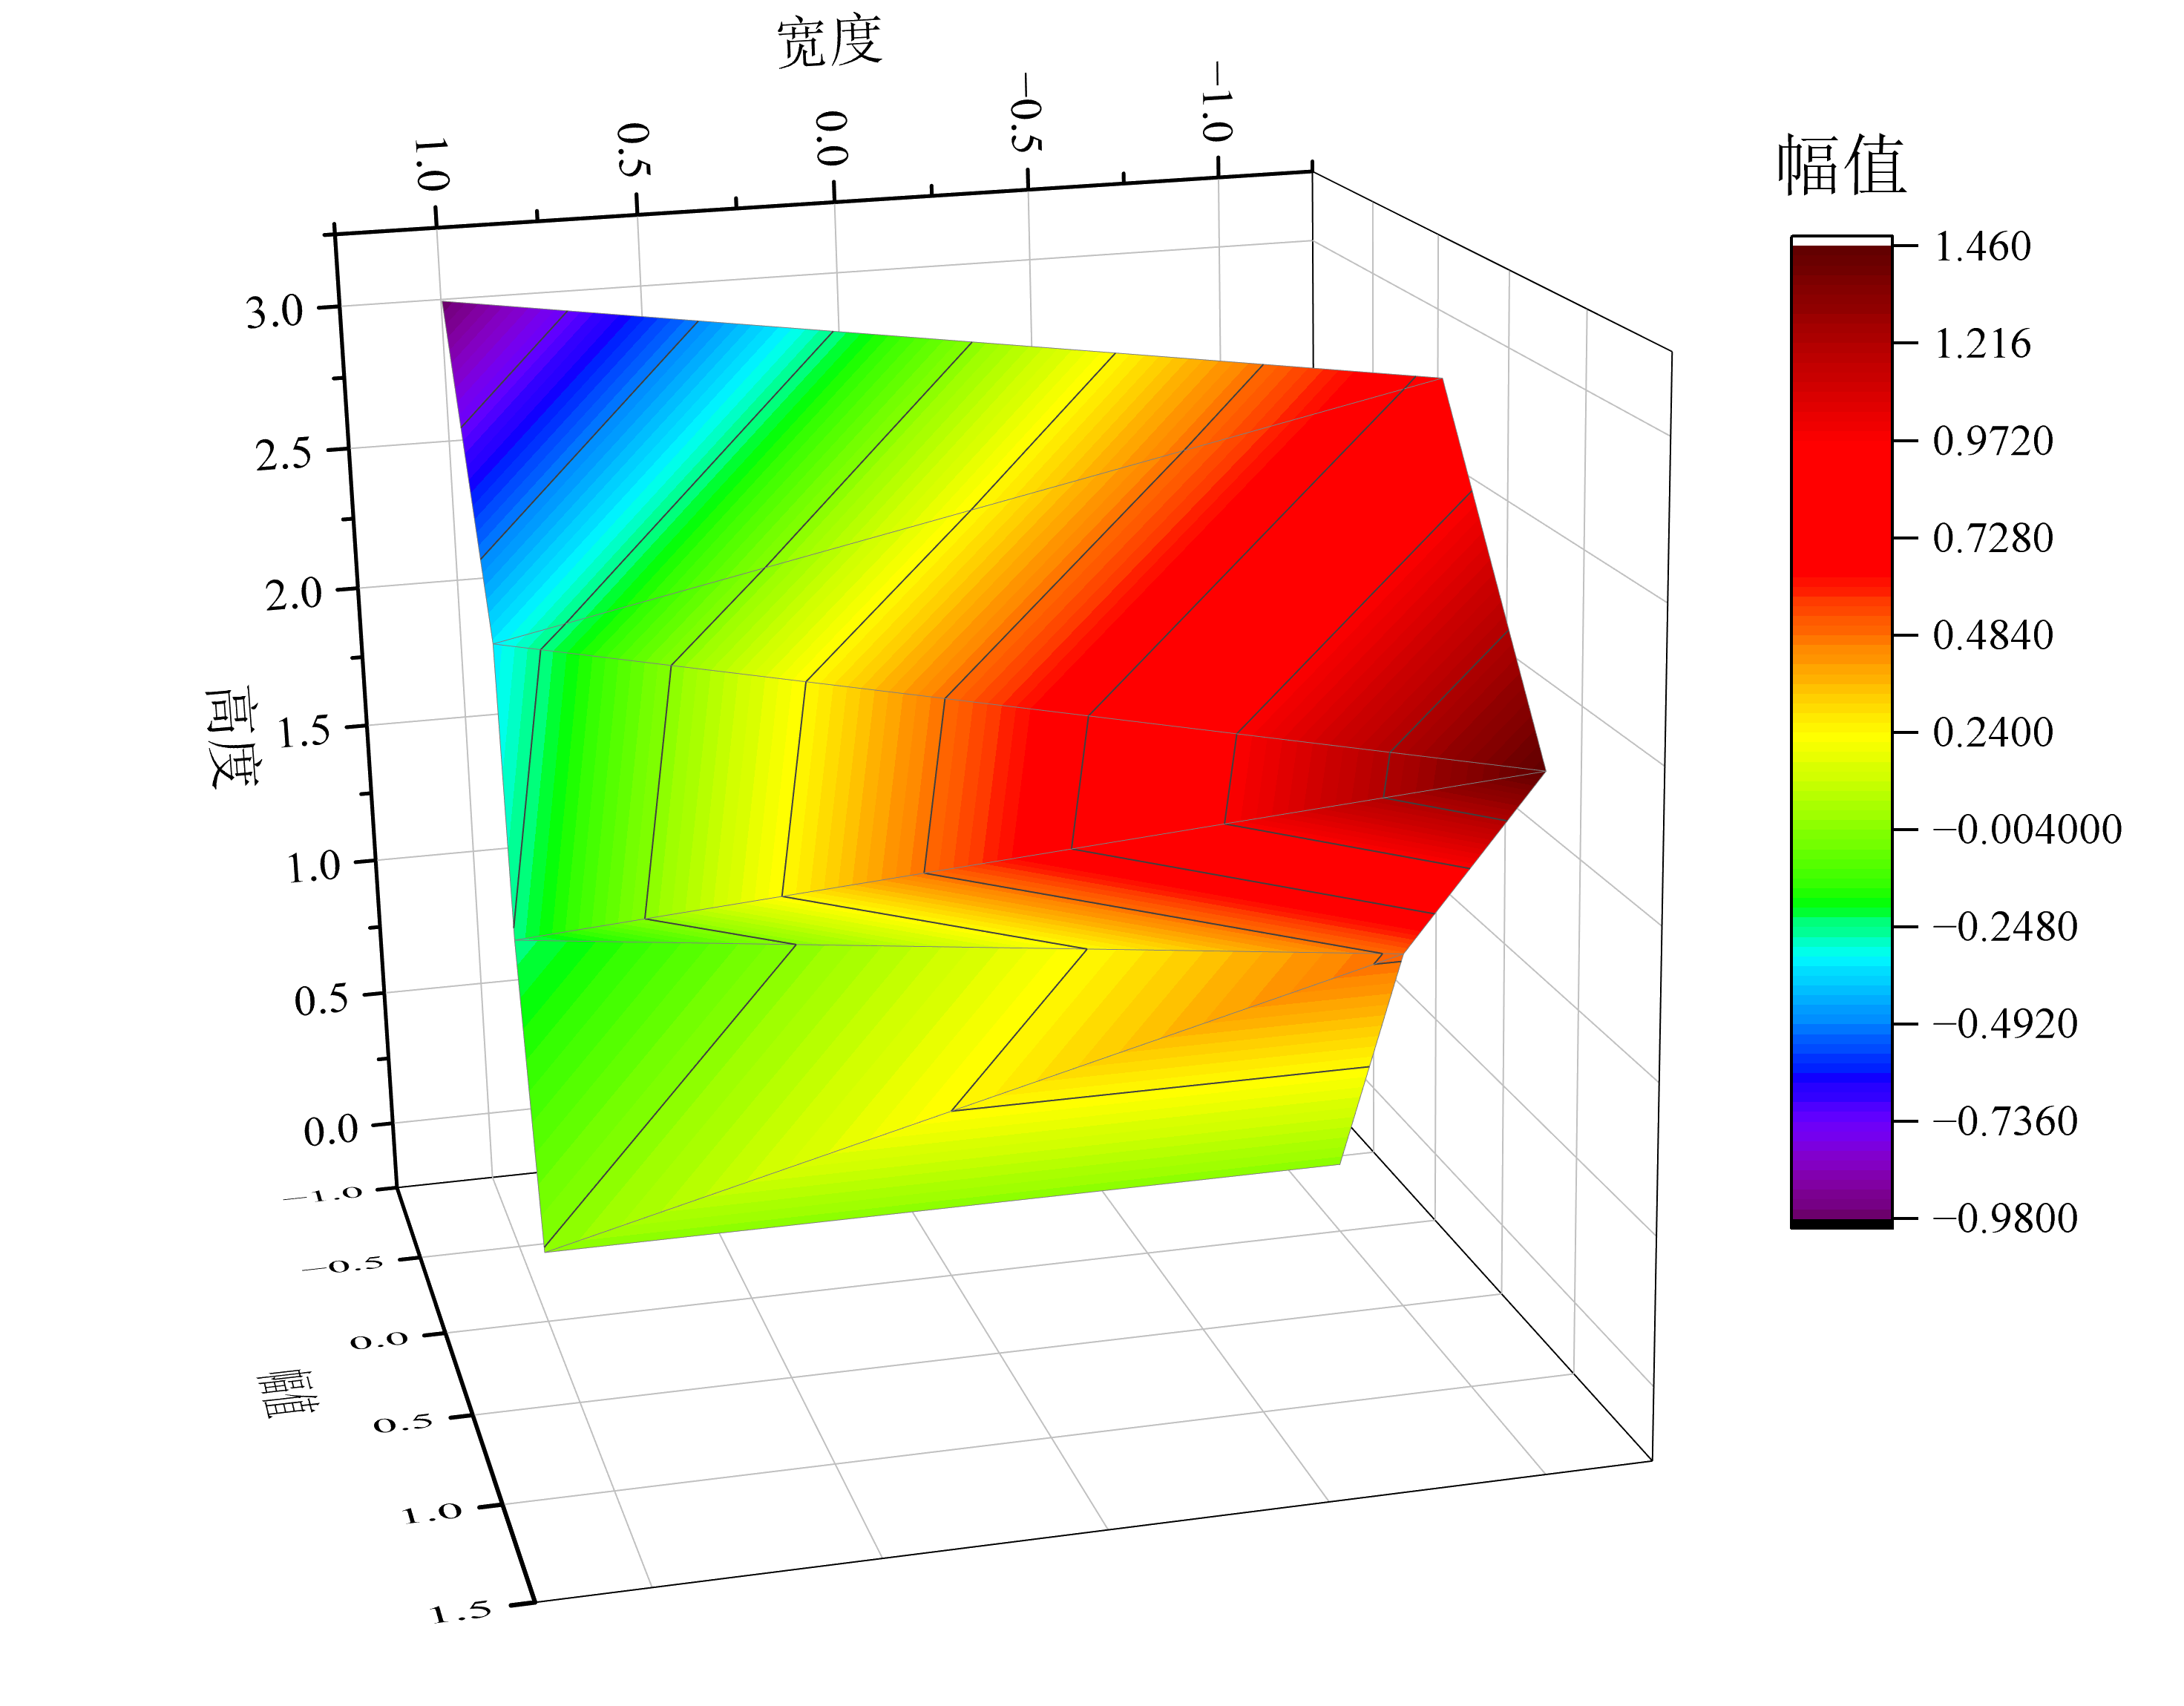
\includegraphics[width=\linewidth]{p14_img01.png}}\hfill
\subcaptionbox{二阶模态}[0.31\textwidth]{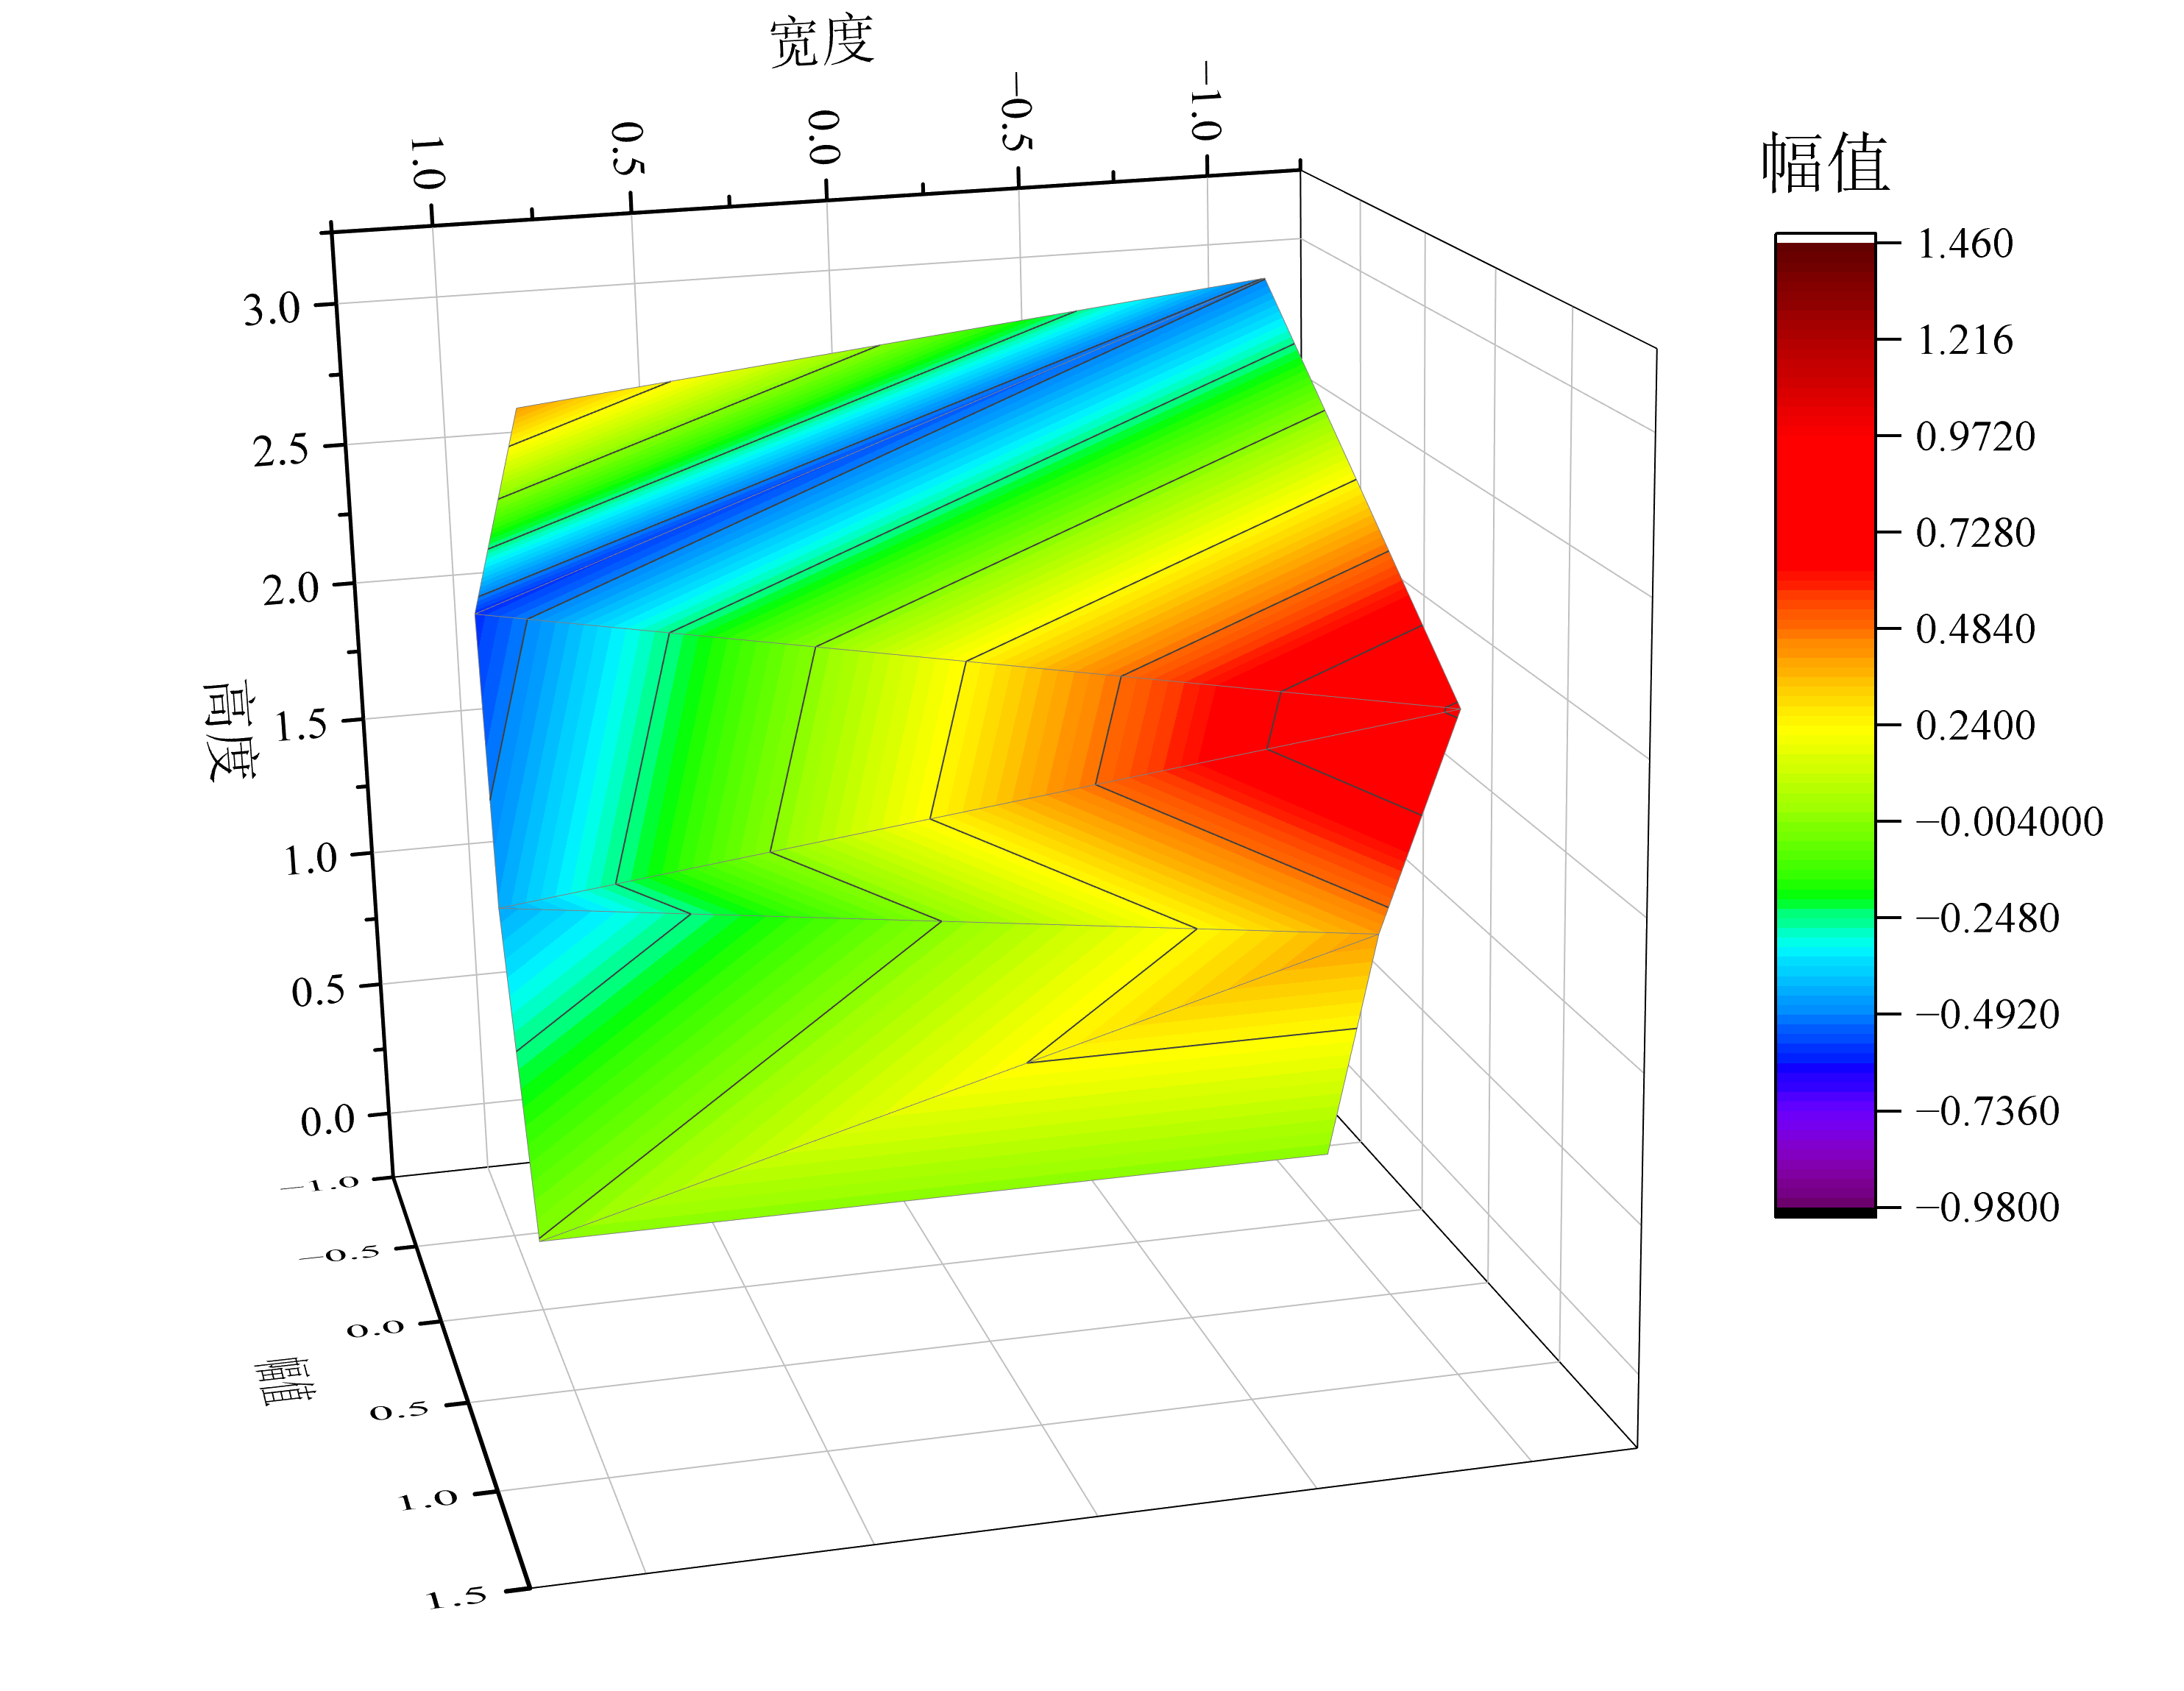
\includegraphics[width=\linewidth]{p14_img02.png}}\hfill
\subcaptionbox{三阶模态}[0.31\textwidth]{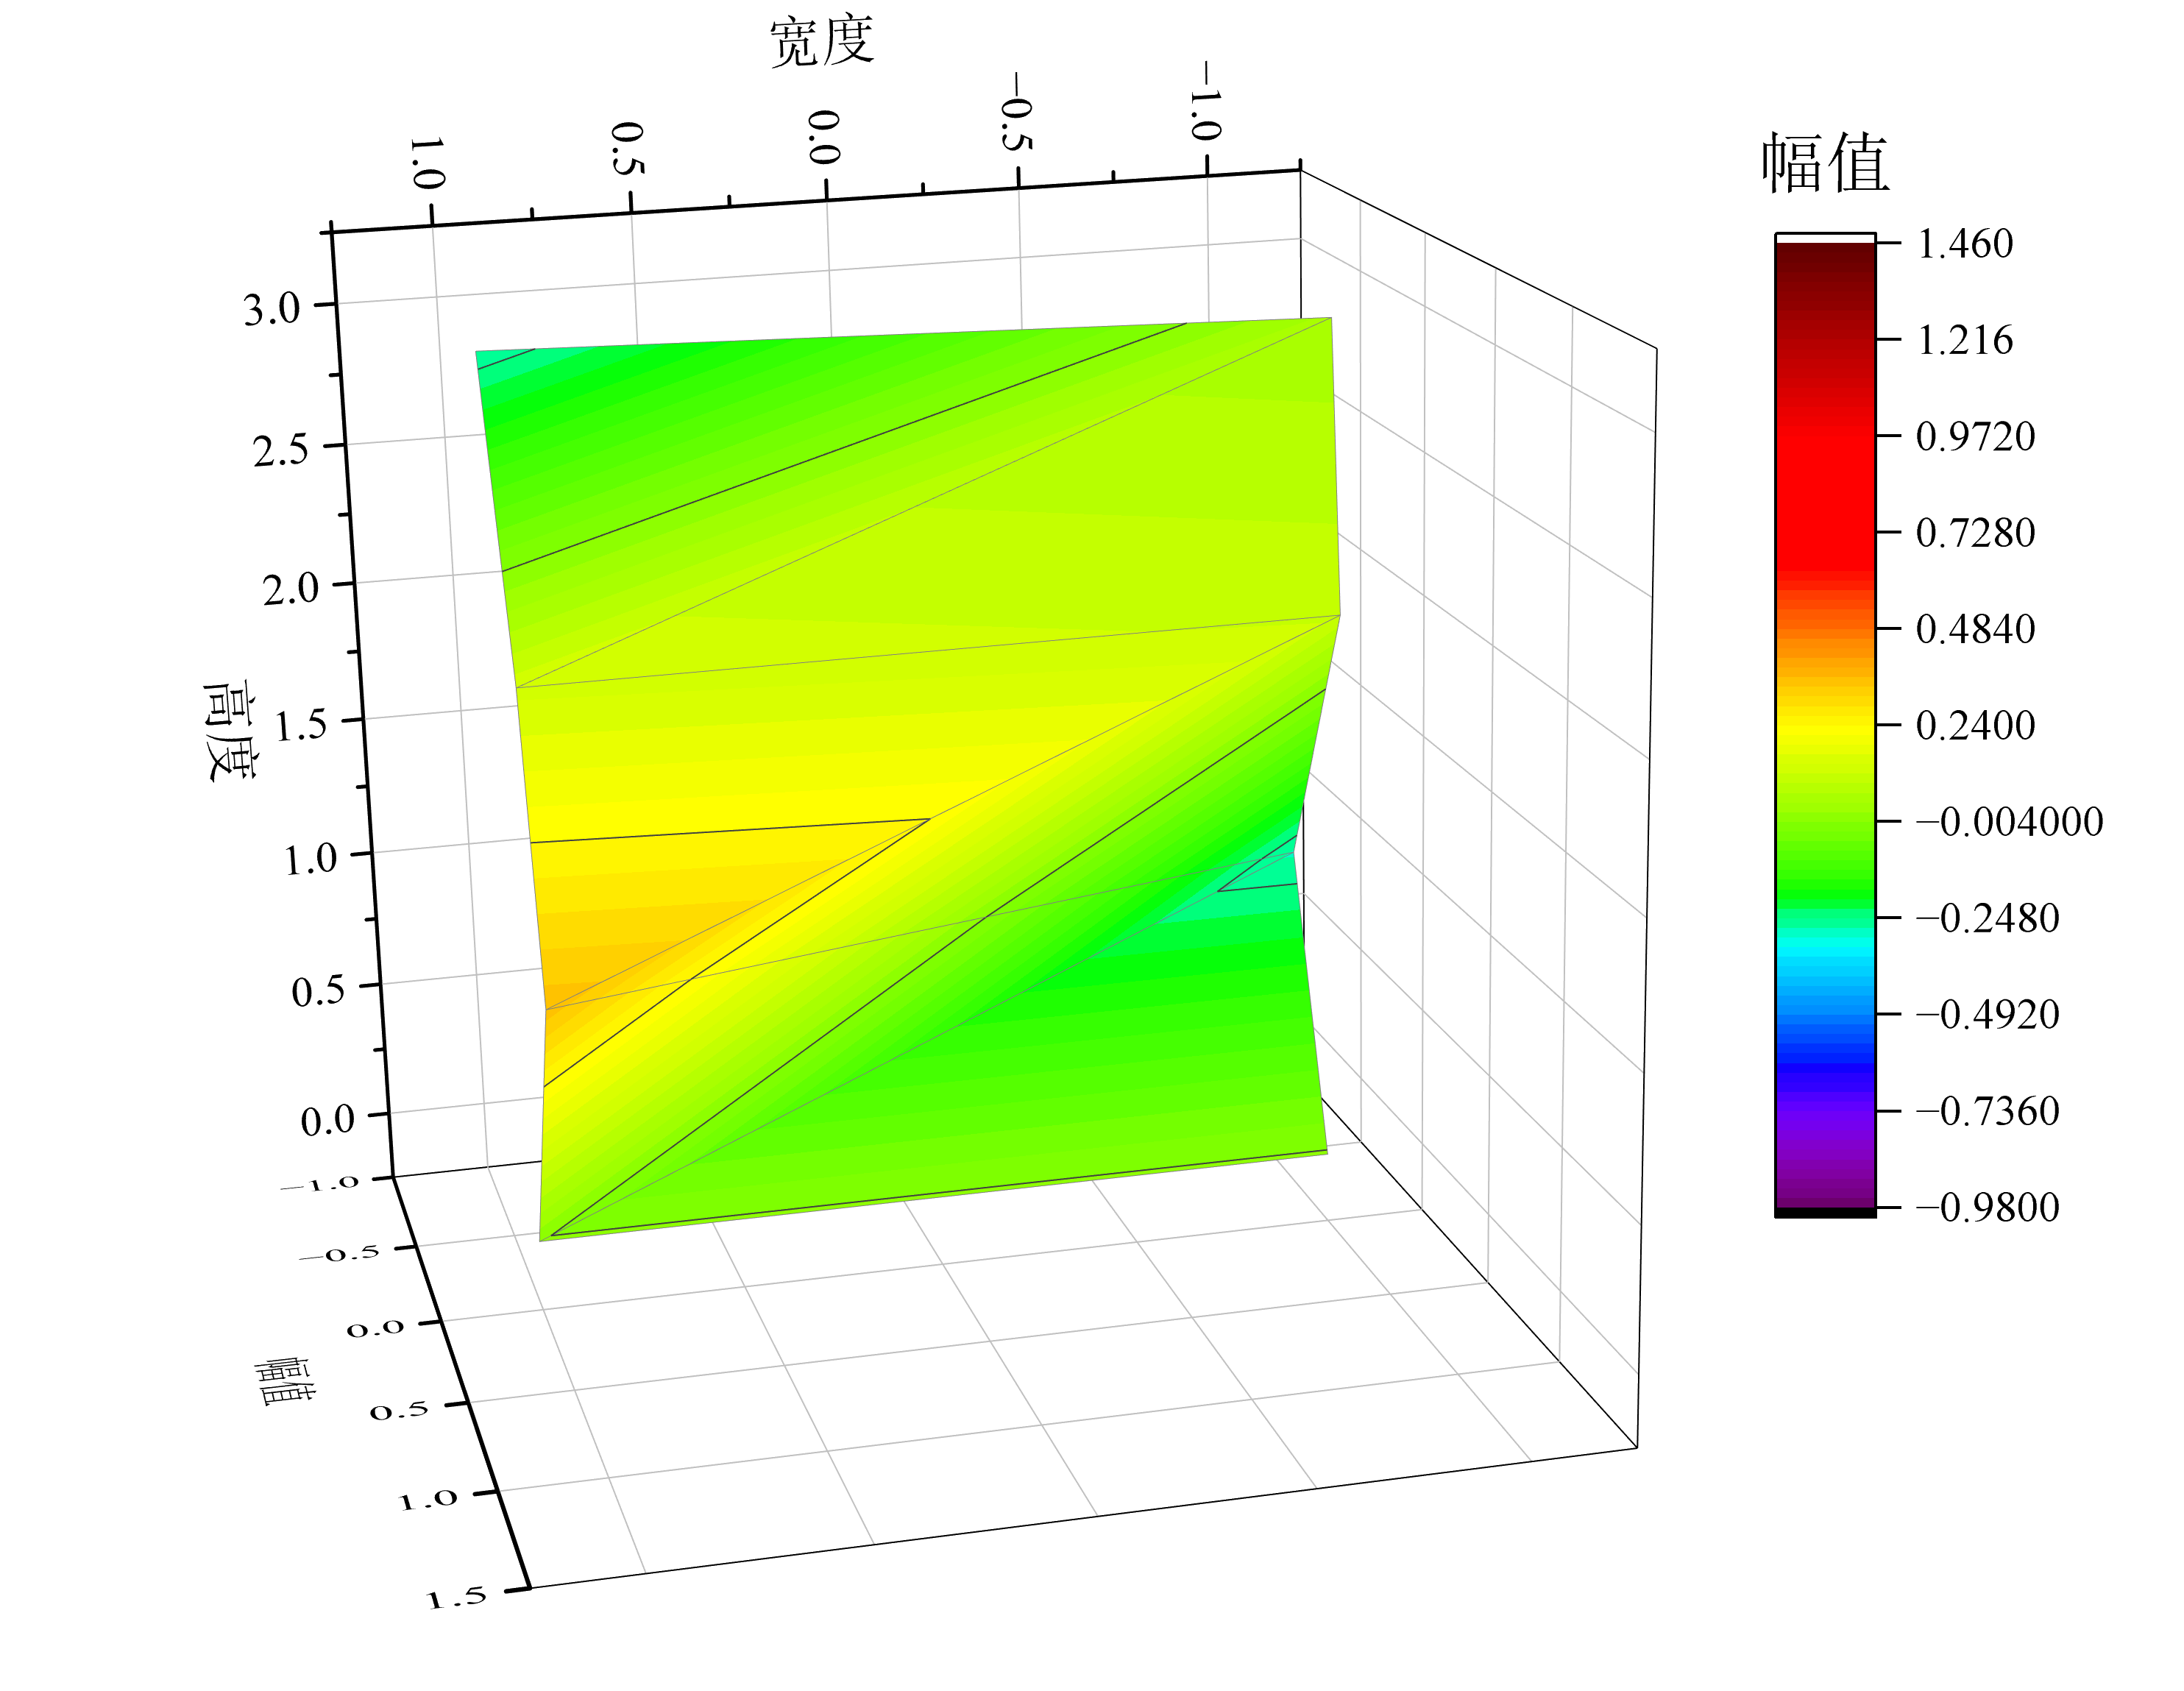
\includegraphics[width=\linewidth]{p14_img03.png}}
\caption{钢锤帽正面锤击 SISO 振型图（三维图）}
\label{fig:exp4-steel-front-mode3d}
\end{figure}

实频函数零点和虚频函数极值点对应固有频率，据此得到扭转振动前三阶固有频率，填入表\ref{tab:exp4-steel-front-frequency}。按式\eqref{eq:exp4-damping}计算阻尼比，填入表\ref{tab:exp4-steel-front-damping}。

\begin{table}[H]
\centering\small
\caption{钢锤帽正面锤击 SISO 前三阶固有频率}
\label{tab:exp4-steel-front-frequency}
\begin{tabular}{lccc}
\toprule
阶数 & 一阶 & 二阶 & 三阶\\
\midrule
锤击1点（Hz） & \blank[1.6cm] & \blank[1.6cm] & \blank[1.6cm]\\
锤击2点（Hz） & \blank[1.6cm] & \blank[1.6cm] & \blank[1.6cm]\\
锤击3点（Hz） & \blank[1.6cm] & \blank[1.6cm] & \blank[1.6cm]\\
锤击4点（Hz） & \blank[1.6cm] & \blank[1.6cm] & \blank[1.6cm]\\
锤击5点（Hz） & \blank[1.6cm] & \blank[1.6cm] & \blank[1.6cm]\\
锤击6点（Hz） & \blank[1.6cm] & \blank[1.6cm] & \blank[1.6cm]\\
平均（Hz） & \blank[1.6cm] & \blank[1.6cm] & \blank[1.6cm]\\
\bottomrule
\end{tabular}
\end{table}

\begin{table}[H]
\centering\small
\caption{钢锤帽正面锤击 SISO 阻尼比}
\label{tab:exp4-steel-front-damping}
\begin{tabular}{lccc}
\toprule
阶数 & 一阶 & 二阶 & 三阶\\
\midrule
锤击1点 & \blank[1.6cm] & \blank[1.6cm] & \blank[1.6cm]\\
锤击2点 & \blank[1.6cm] & \blank[1.6cm] & \blank[1.6cm]\\
锤击3点 & \blank[1.6cm] & \blank[1.6cm] & \blank[1.6cm]\\
锤击4点 & \blank[1.6cm] & \blank[1.6cm] & \blank[1.6cm]\\
锤击5点 & \blank[1.6cm] & \blank[1.6cm] & \blank[1.6cm]\\
锤击6点 & \blank[1.6cm] & \blank[1.6cm] & \blank[1.6cm]\\
平均 & \blank[1.6cm] & \blank[1.6cm] & \blank[1.6cm]\\
\bottomrule
\end{tabular}
\end{table}

\subsubsection{钢锤帽侧面锤击}
力锤选用钢锤帽，分别在模型侧面锤击“10”“11”“12”“16”“17”“18”号位置，通过多次测试，在模型正面的 B 点测得响应信号。通过 FFT 得到平均后的频响函数，如图\ref{fig:exp4-steel-side-frf1}和图\ref{fig:exp4-steel-side-frf2}所示。

\begin{figure}[H]
\centering
\subcaptionbox{平均幅频曲线}[0.47\textwidth]{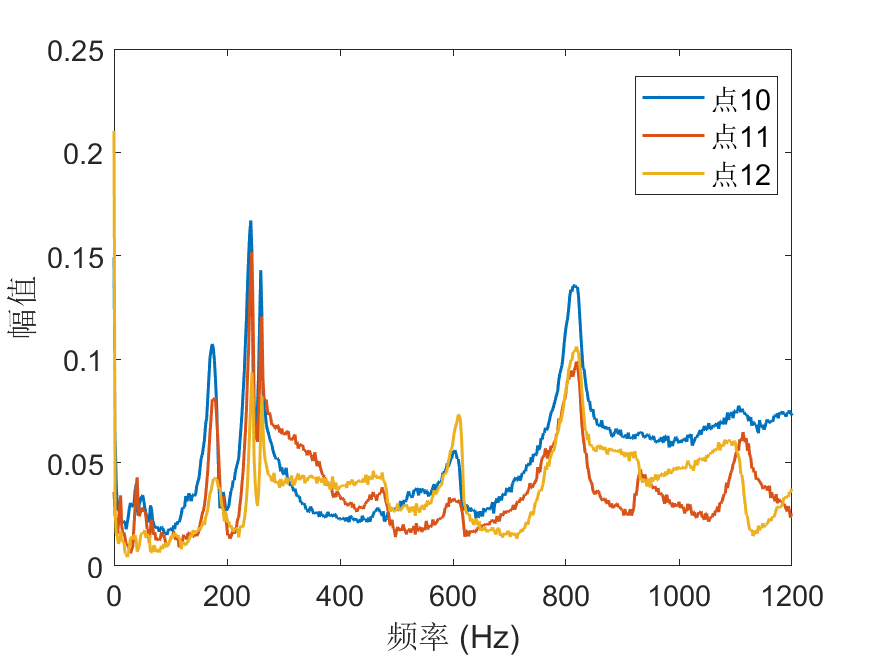
\includegraphics[width=\linewidth]{p15_img01.png}}\hfill
\subcaptionbox{平均实频曲线}[0.47\textwidth]{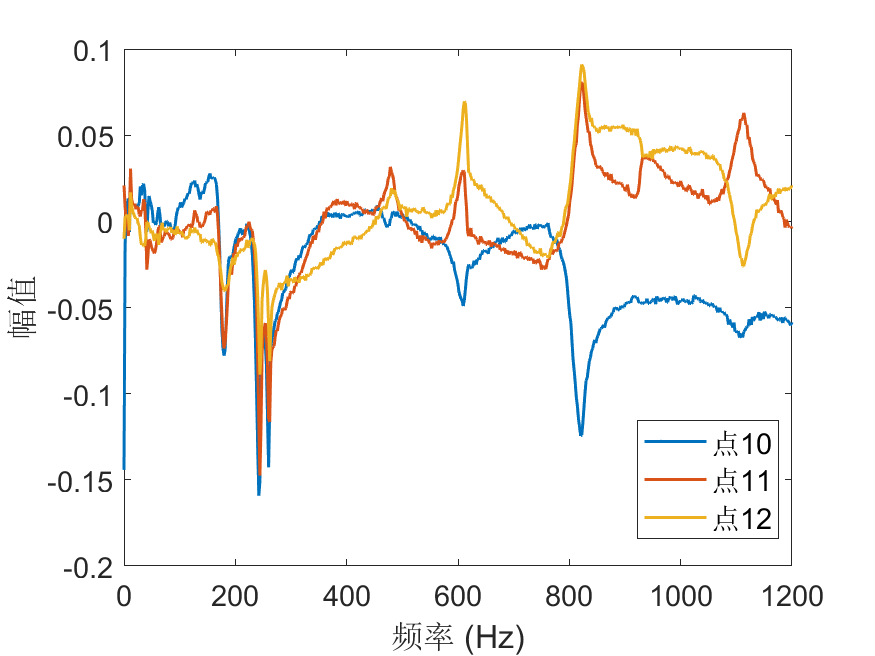
\includegraphics[width=\linewidth]{p15_img02.png}}\\[0.5em]
\subcaptionbox{平均虚频曲线}[0.47\textwidth]{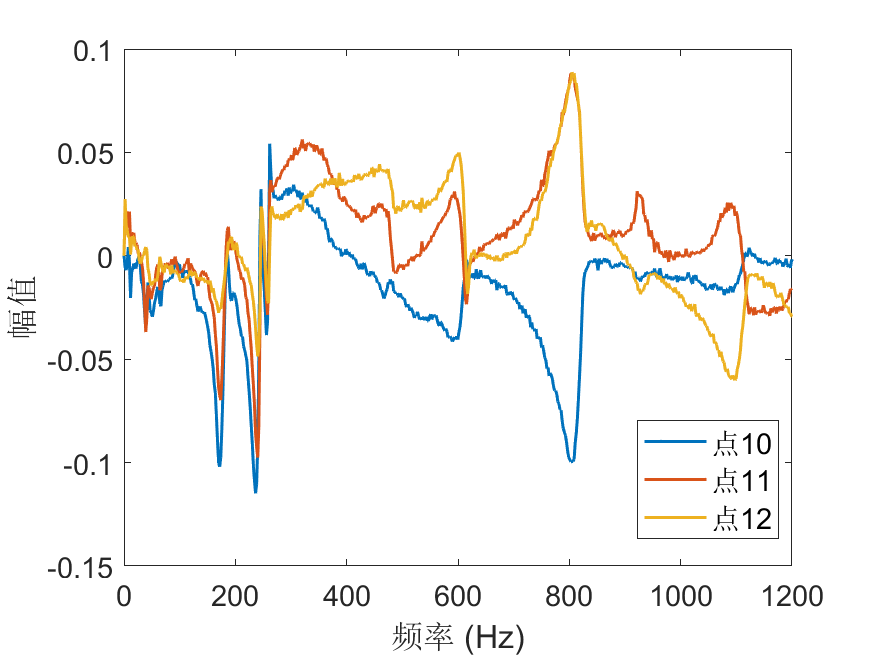
\includegraphics[width=\linewidth]{p15_img03.png}}\hfill
\subcaptionbox{平均相频曲线}[0.47\textwidth]{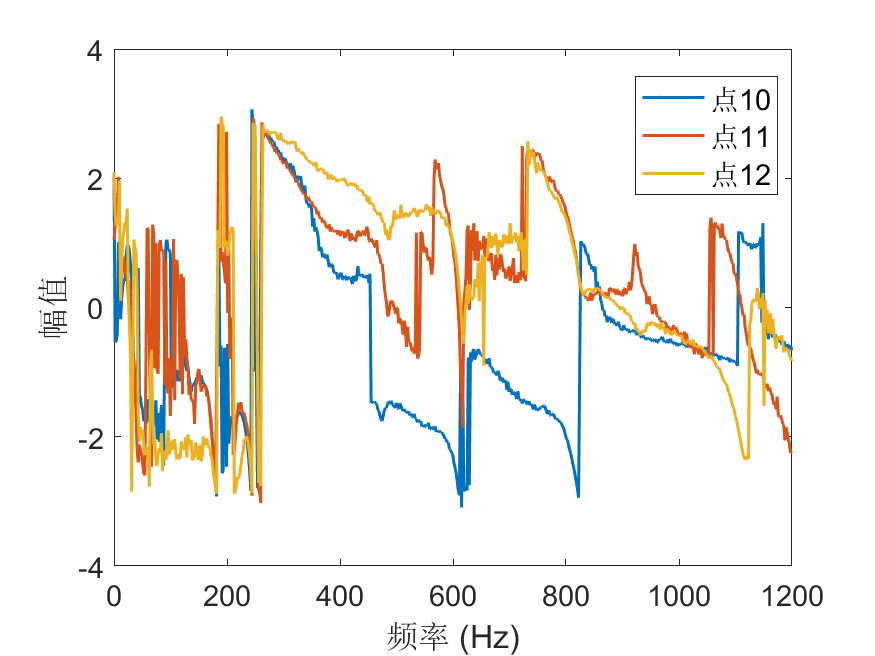
\includegraphics[width=\linewidth]{p15_img04.png}}
\caption{钢锤帽侧面锤击 SISO 频响函数曲线（点10、11、12）}
\label{fig:exp4-steel-side-frf1}
\end{figure}

将点 12 与点 18 对应的幅值归一化为 1，绘制成比例的幅值图。图\ref{fig:exp4-steel-side-mode2d}为位于同一竖直线上的点构成的模态图，图\ref{fig:exp4-steel-side-mode3d}为完整三维模态图。

\begin{figure}[H]
\centering
\subcaptionbox{平均幅频曲线}[0.47\textwidth]{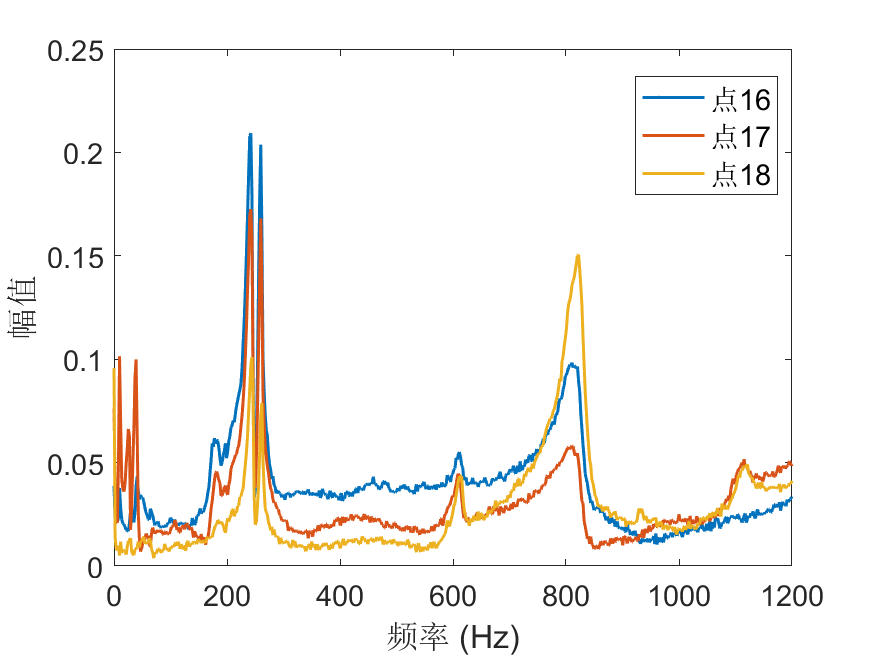
\includegraphics[width=\linewidth]{p16_img01.png}}\hfill
\subcaptionbox{平均实频曲线}[0.47\textwidth]{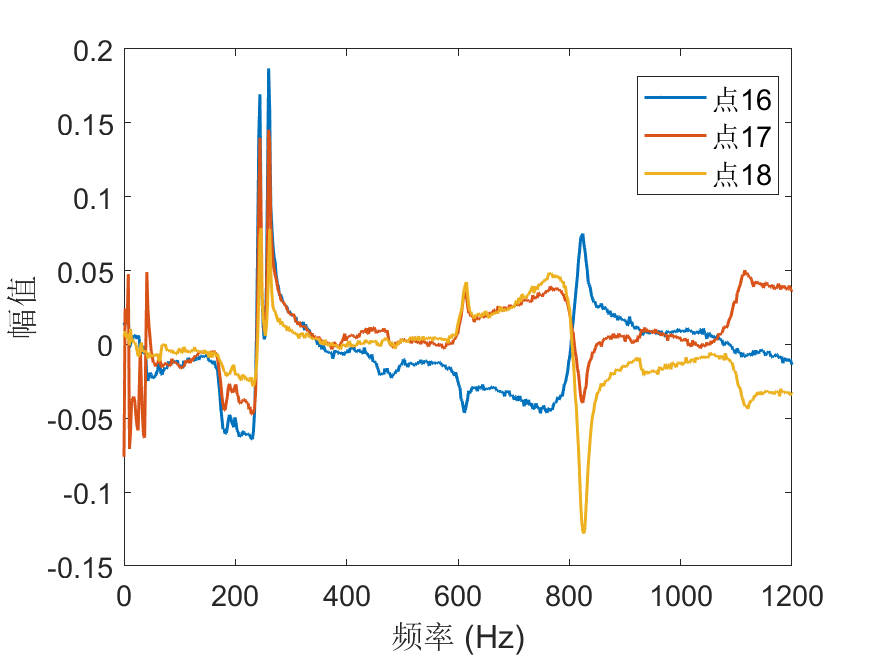
\includegraphics[width=\linewidth]{p16_img02.png}}\\[0.5em]
\subcaptionbox{平均虚频曲线}[0.47\textwidth]{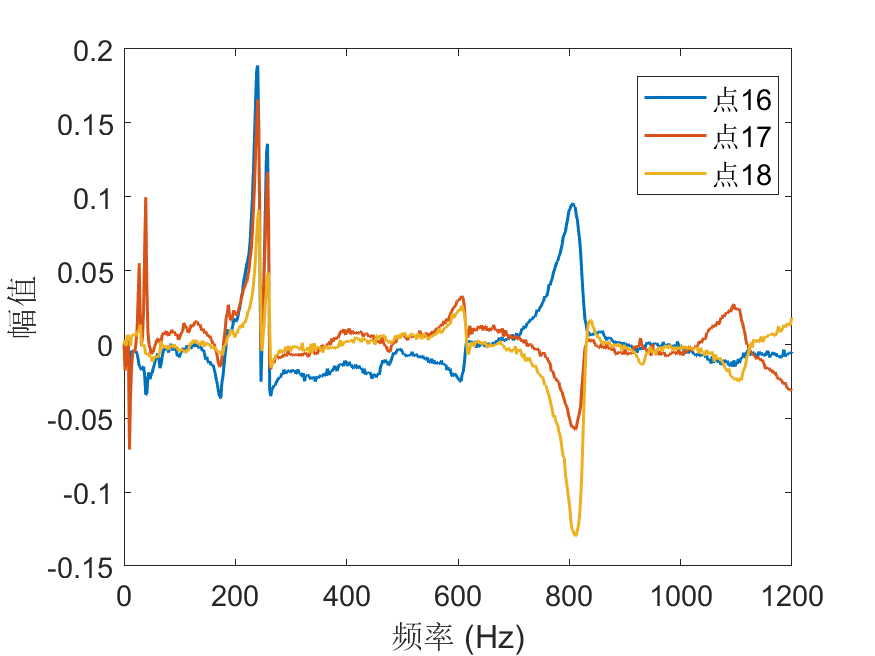
\includegraphics[width=\linewidth]{p16_img03.png}}\hfill
\subcaptionbox{平均相频曲线}[0.47\textwidth]{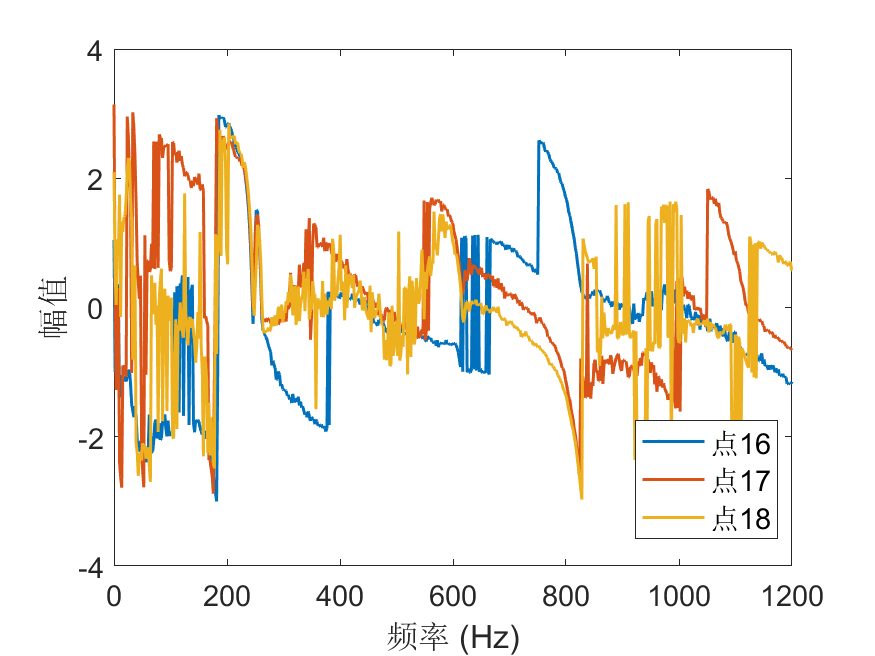
\includegraphics[width=\linewidth]{p16_img04.png}}
\caption{钢锤帽侧面锤击 SISO 频响函数曲线（点16、17、18）}
\label{fig:exp4-steel-side-frf2}
\end{figure}

\begin{figure}[H]
\centering
\subcaptionbox{点10、11、12}[0.47\textwidth]{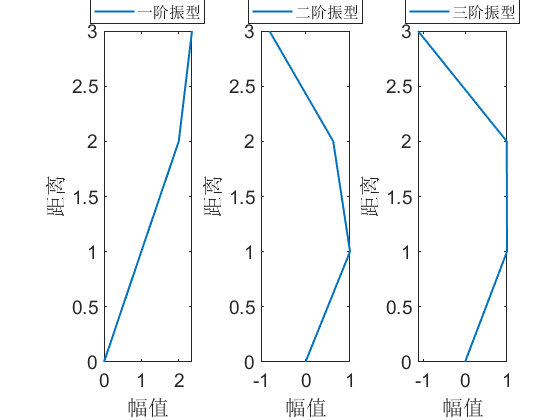
\includegraphics[width=\linewidth]{p16_img05.png}}\hfill
\subcaptionbox{点16、17、18}[0.47\textwidth]{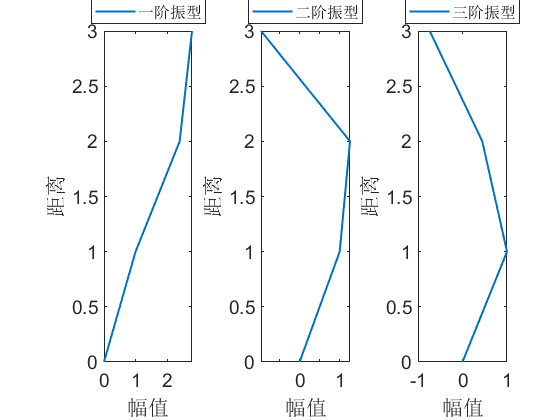
\includegraphics[width=\linewidth]{p16_img06.png}}
\caption{钢锤帽侧面锤击 SISO 振型图}
\label{fig:exp4-steel-side-mode2d}
\end{figure}

\begin{figure}[H]
\centering
\subcaptionbox{一阶模态}[0.31\textwidth]{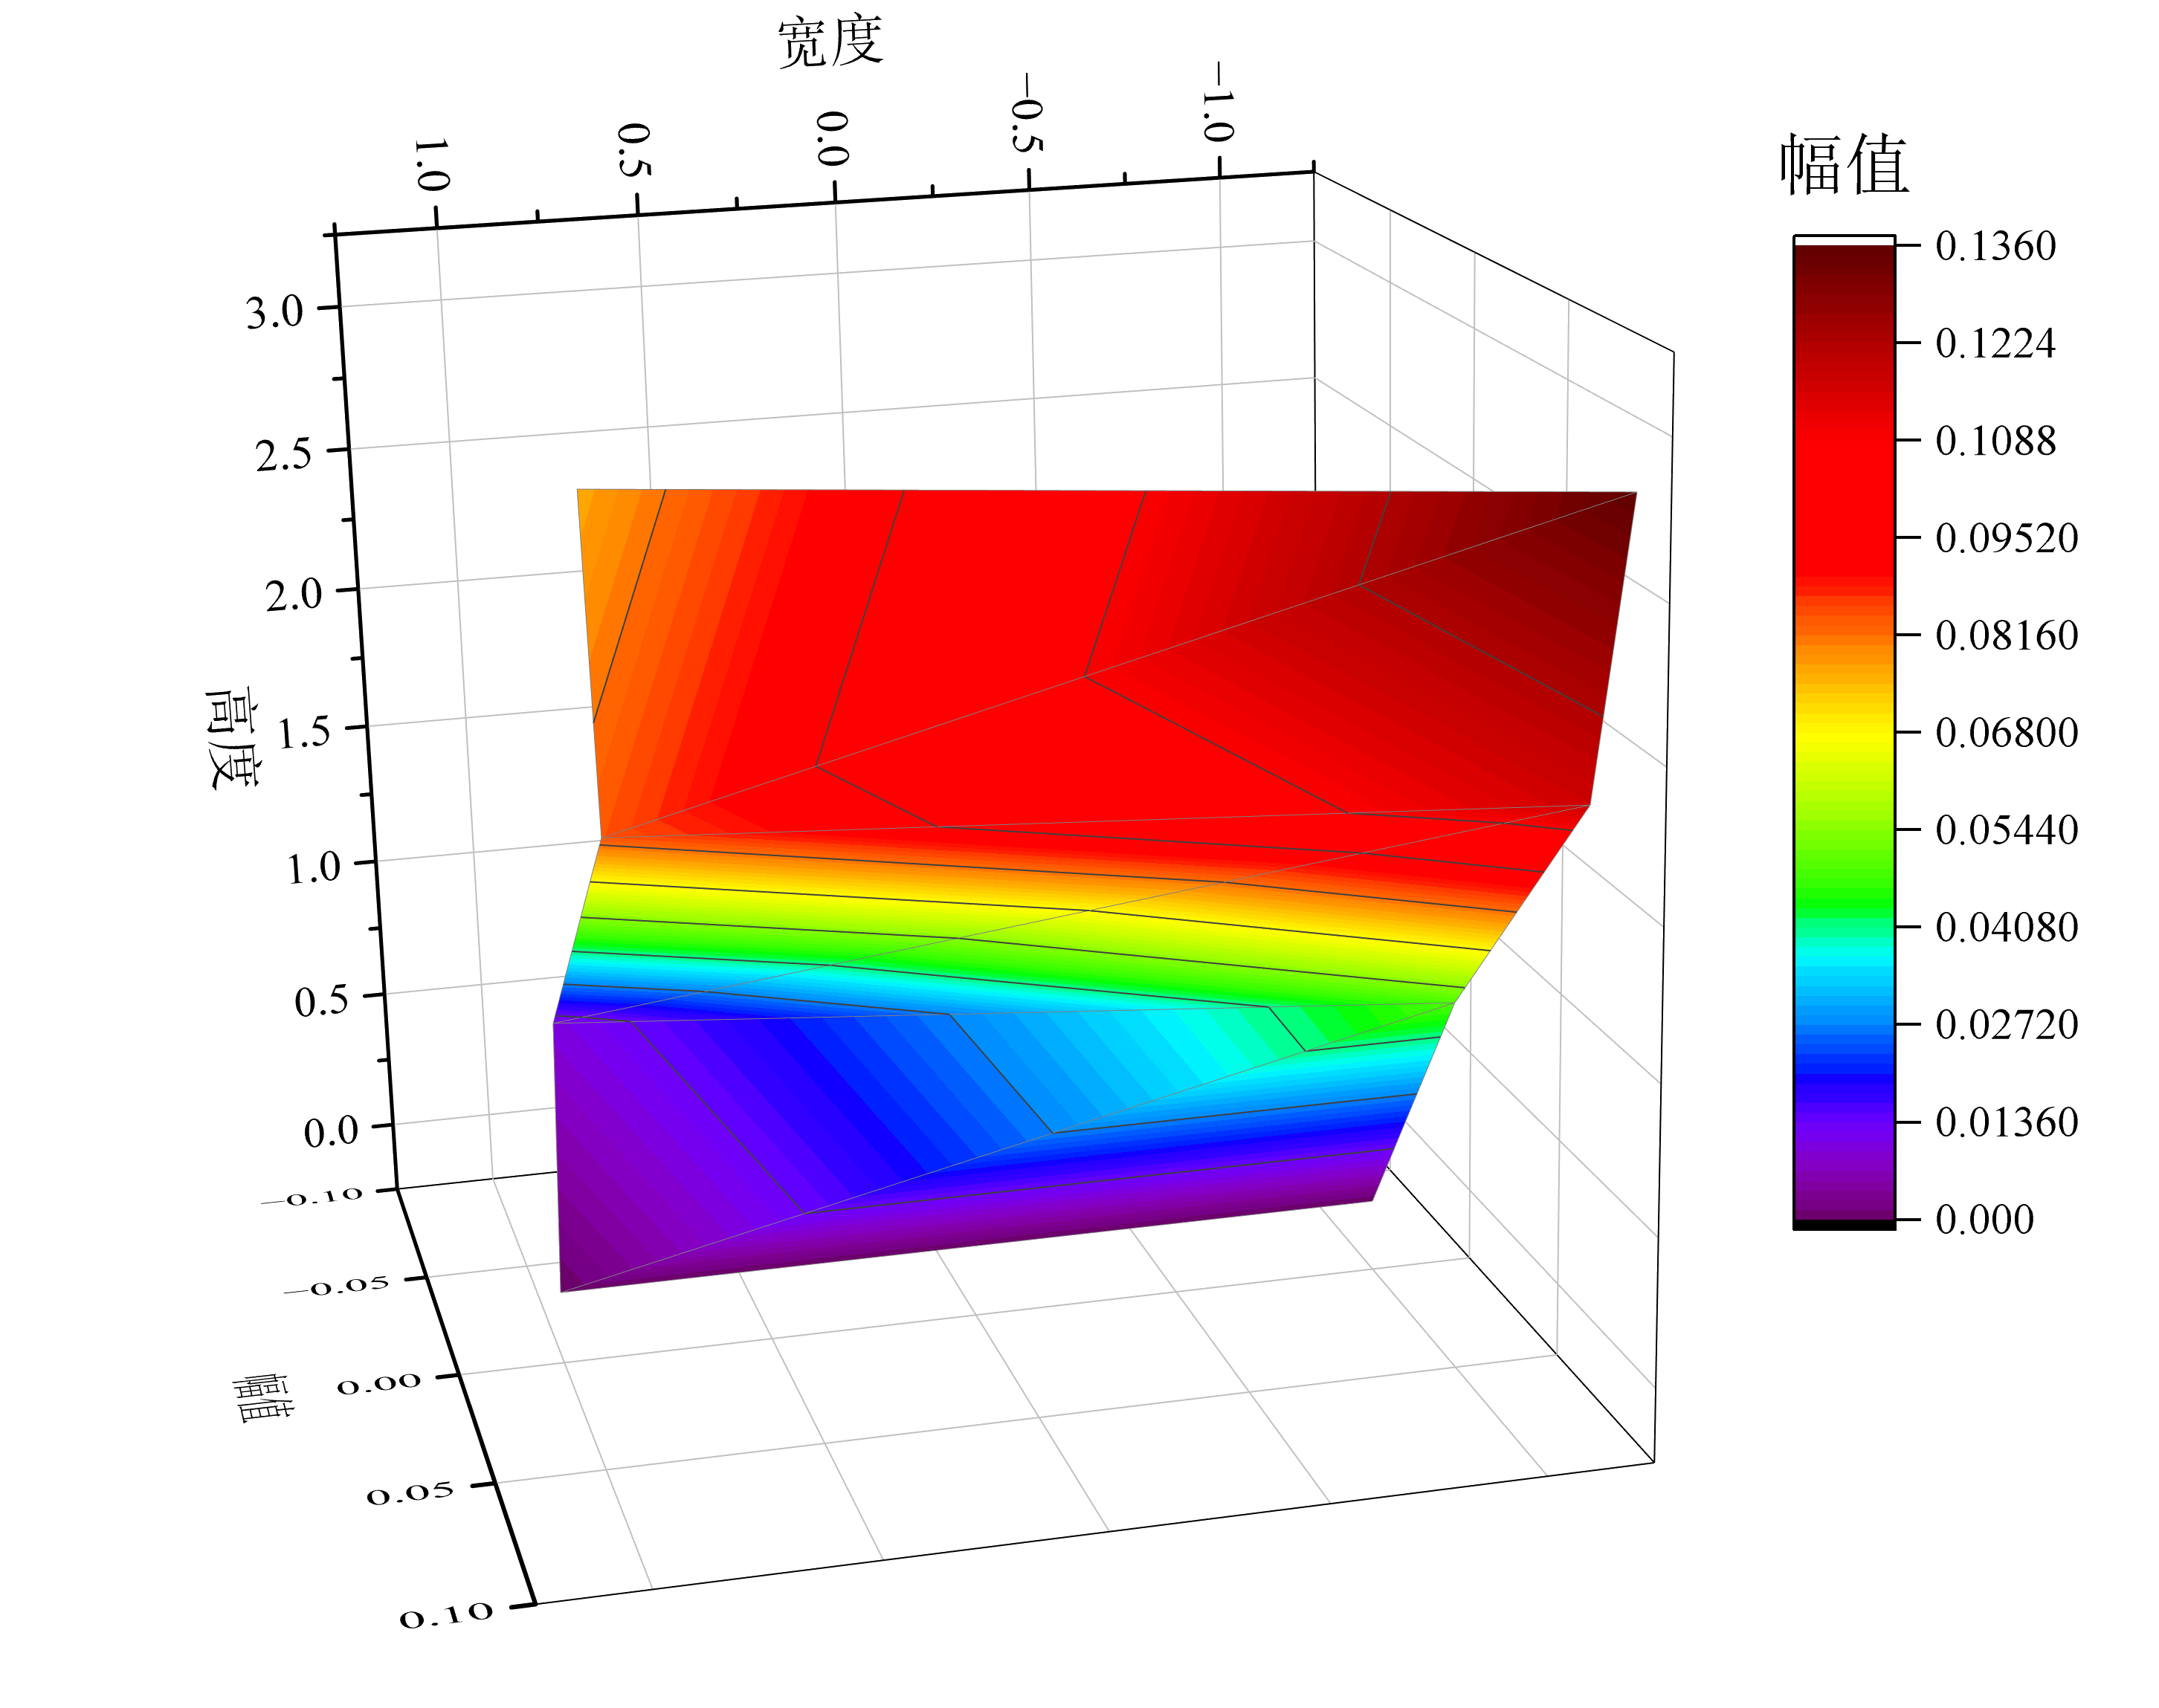
\includegraphics[width=\linewidth]{p17_img01.png}}\hfill
\subcaptionbox{二阶模态}[0.31\textwidth]{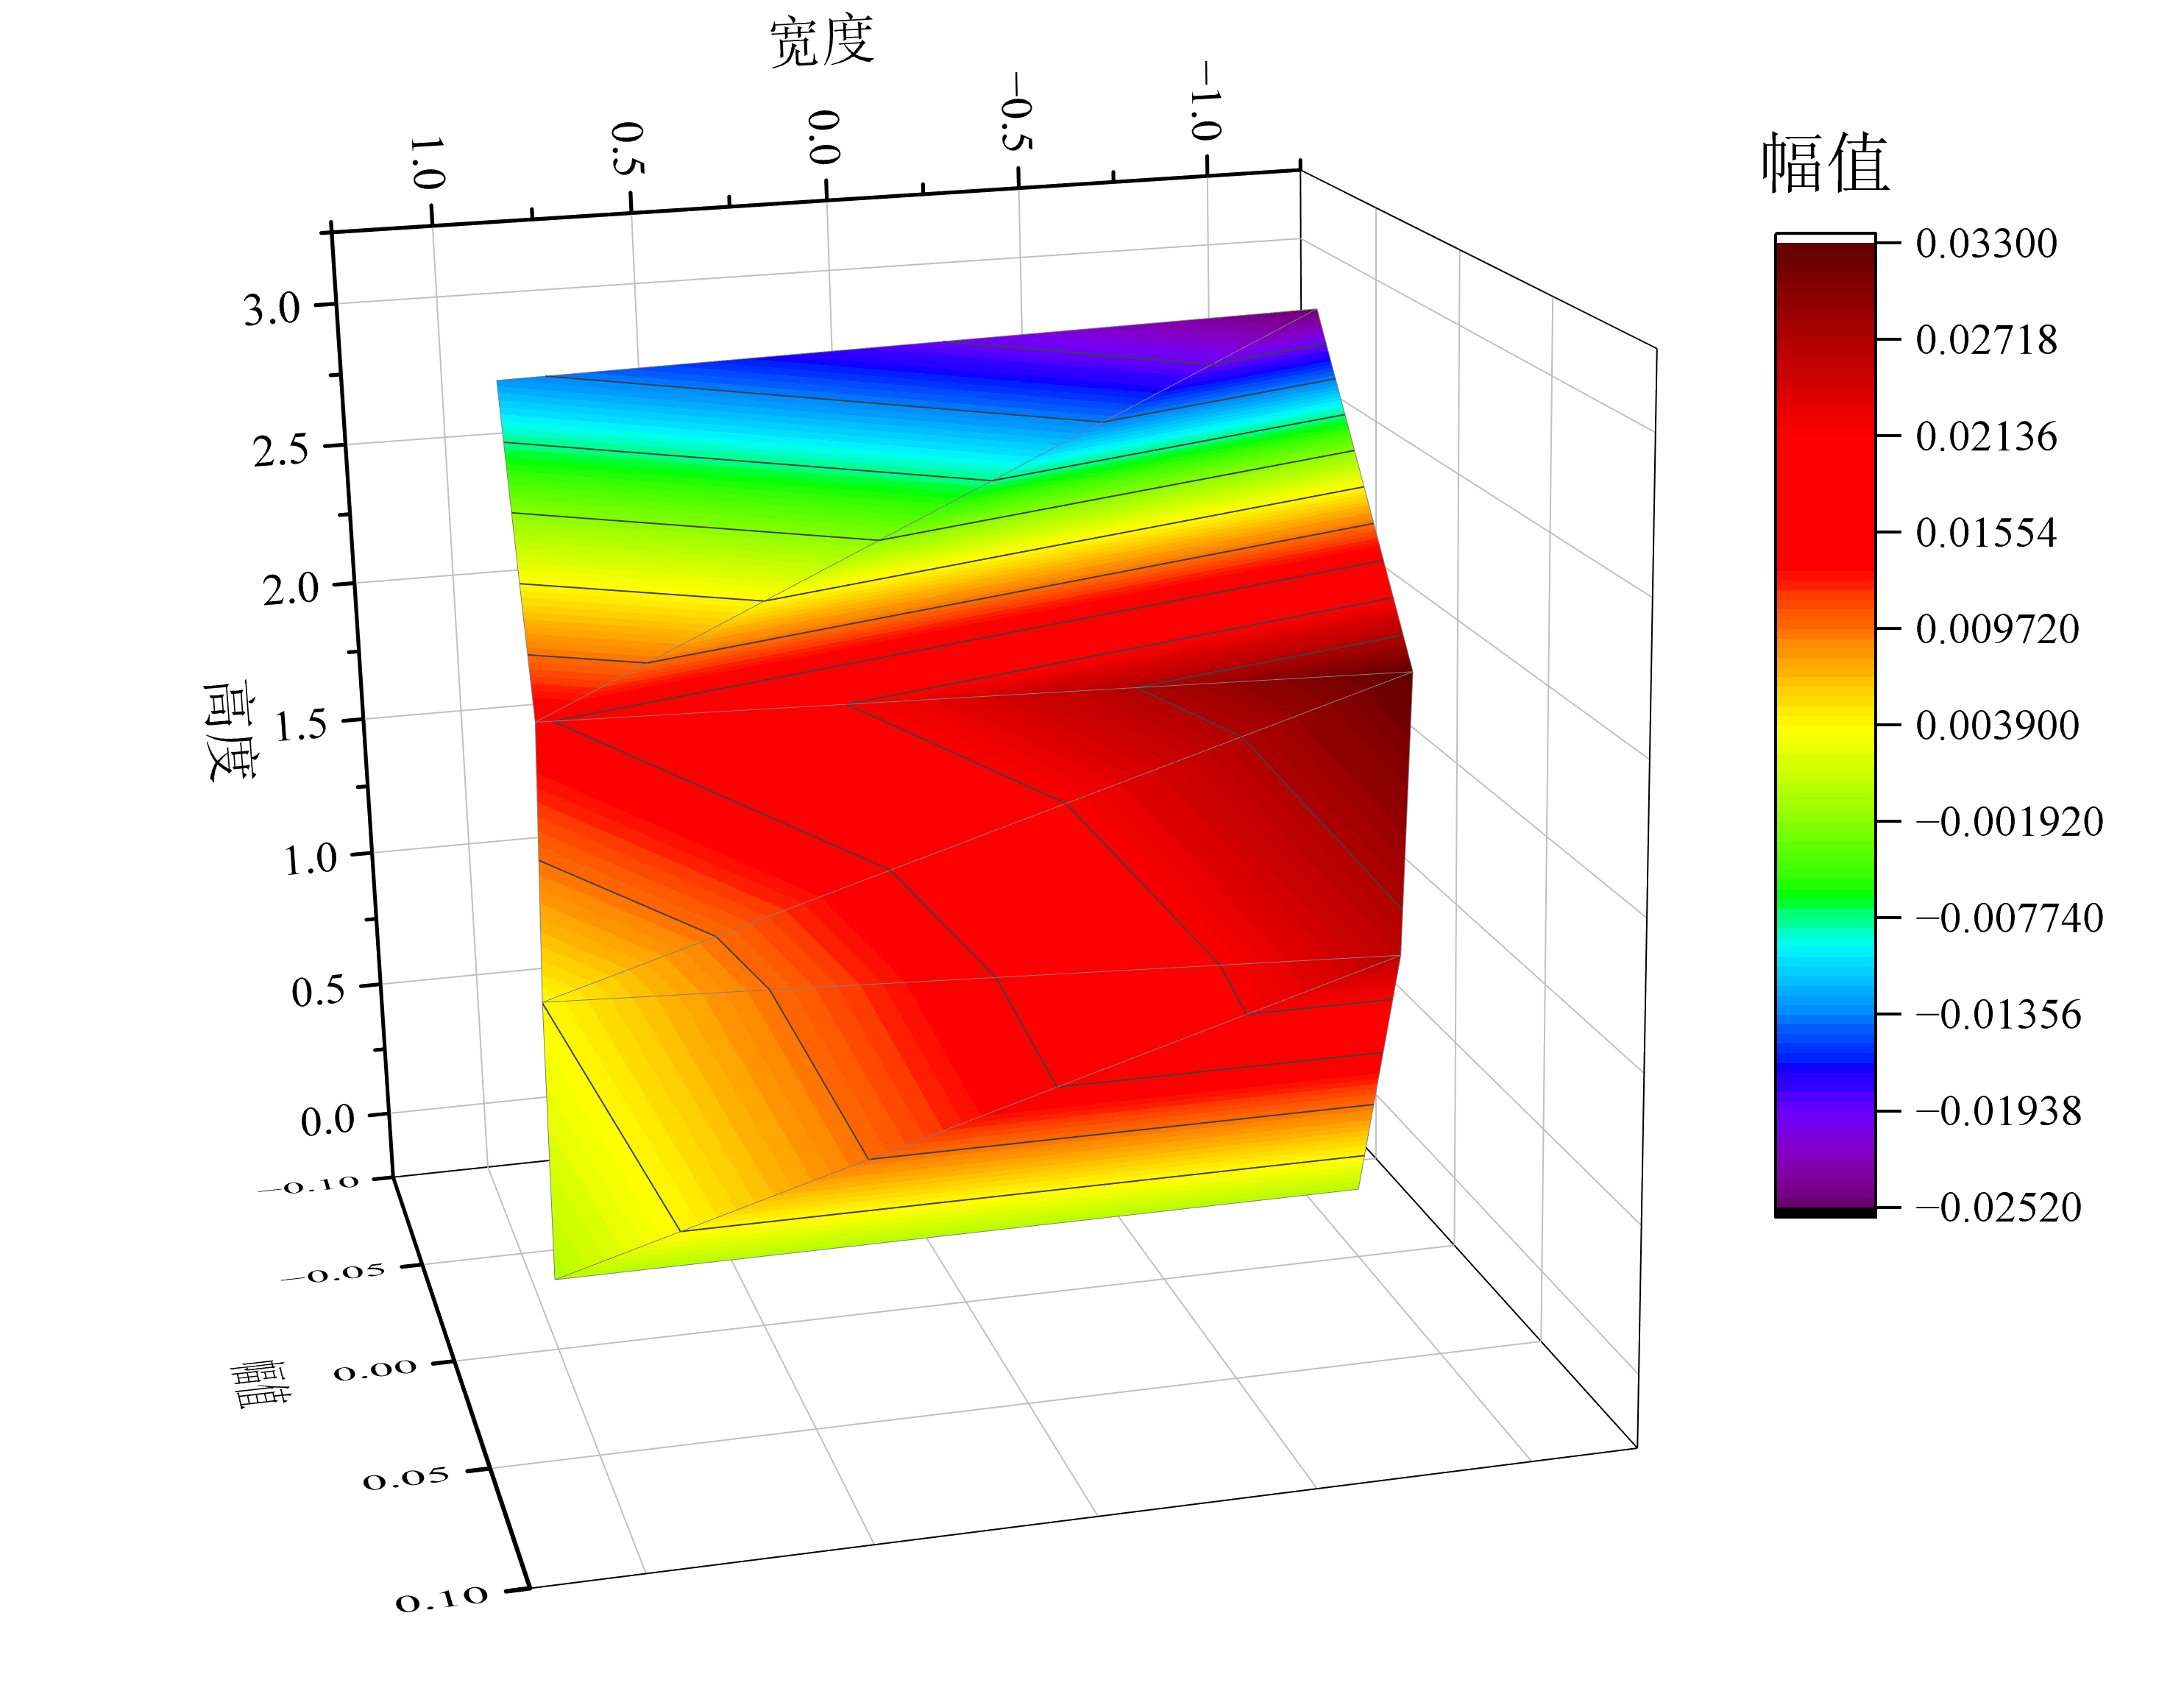
\includegraphics[width=\linewidth]{p17_img02.png}}\hfill
\subcaptionbox{三阶模态}[0.31\textwidth]{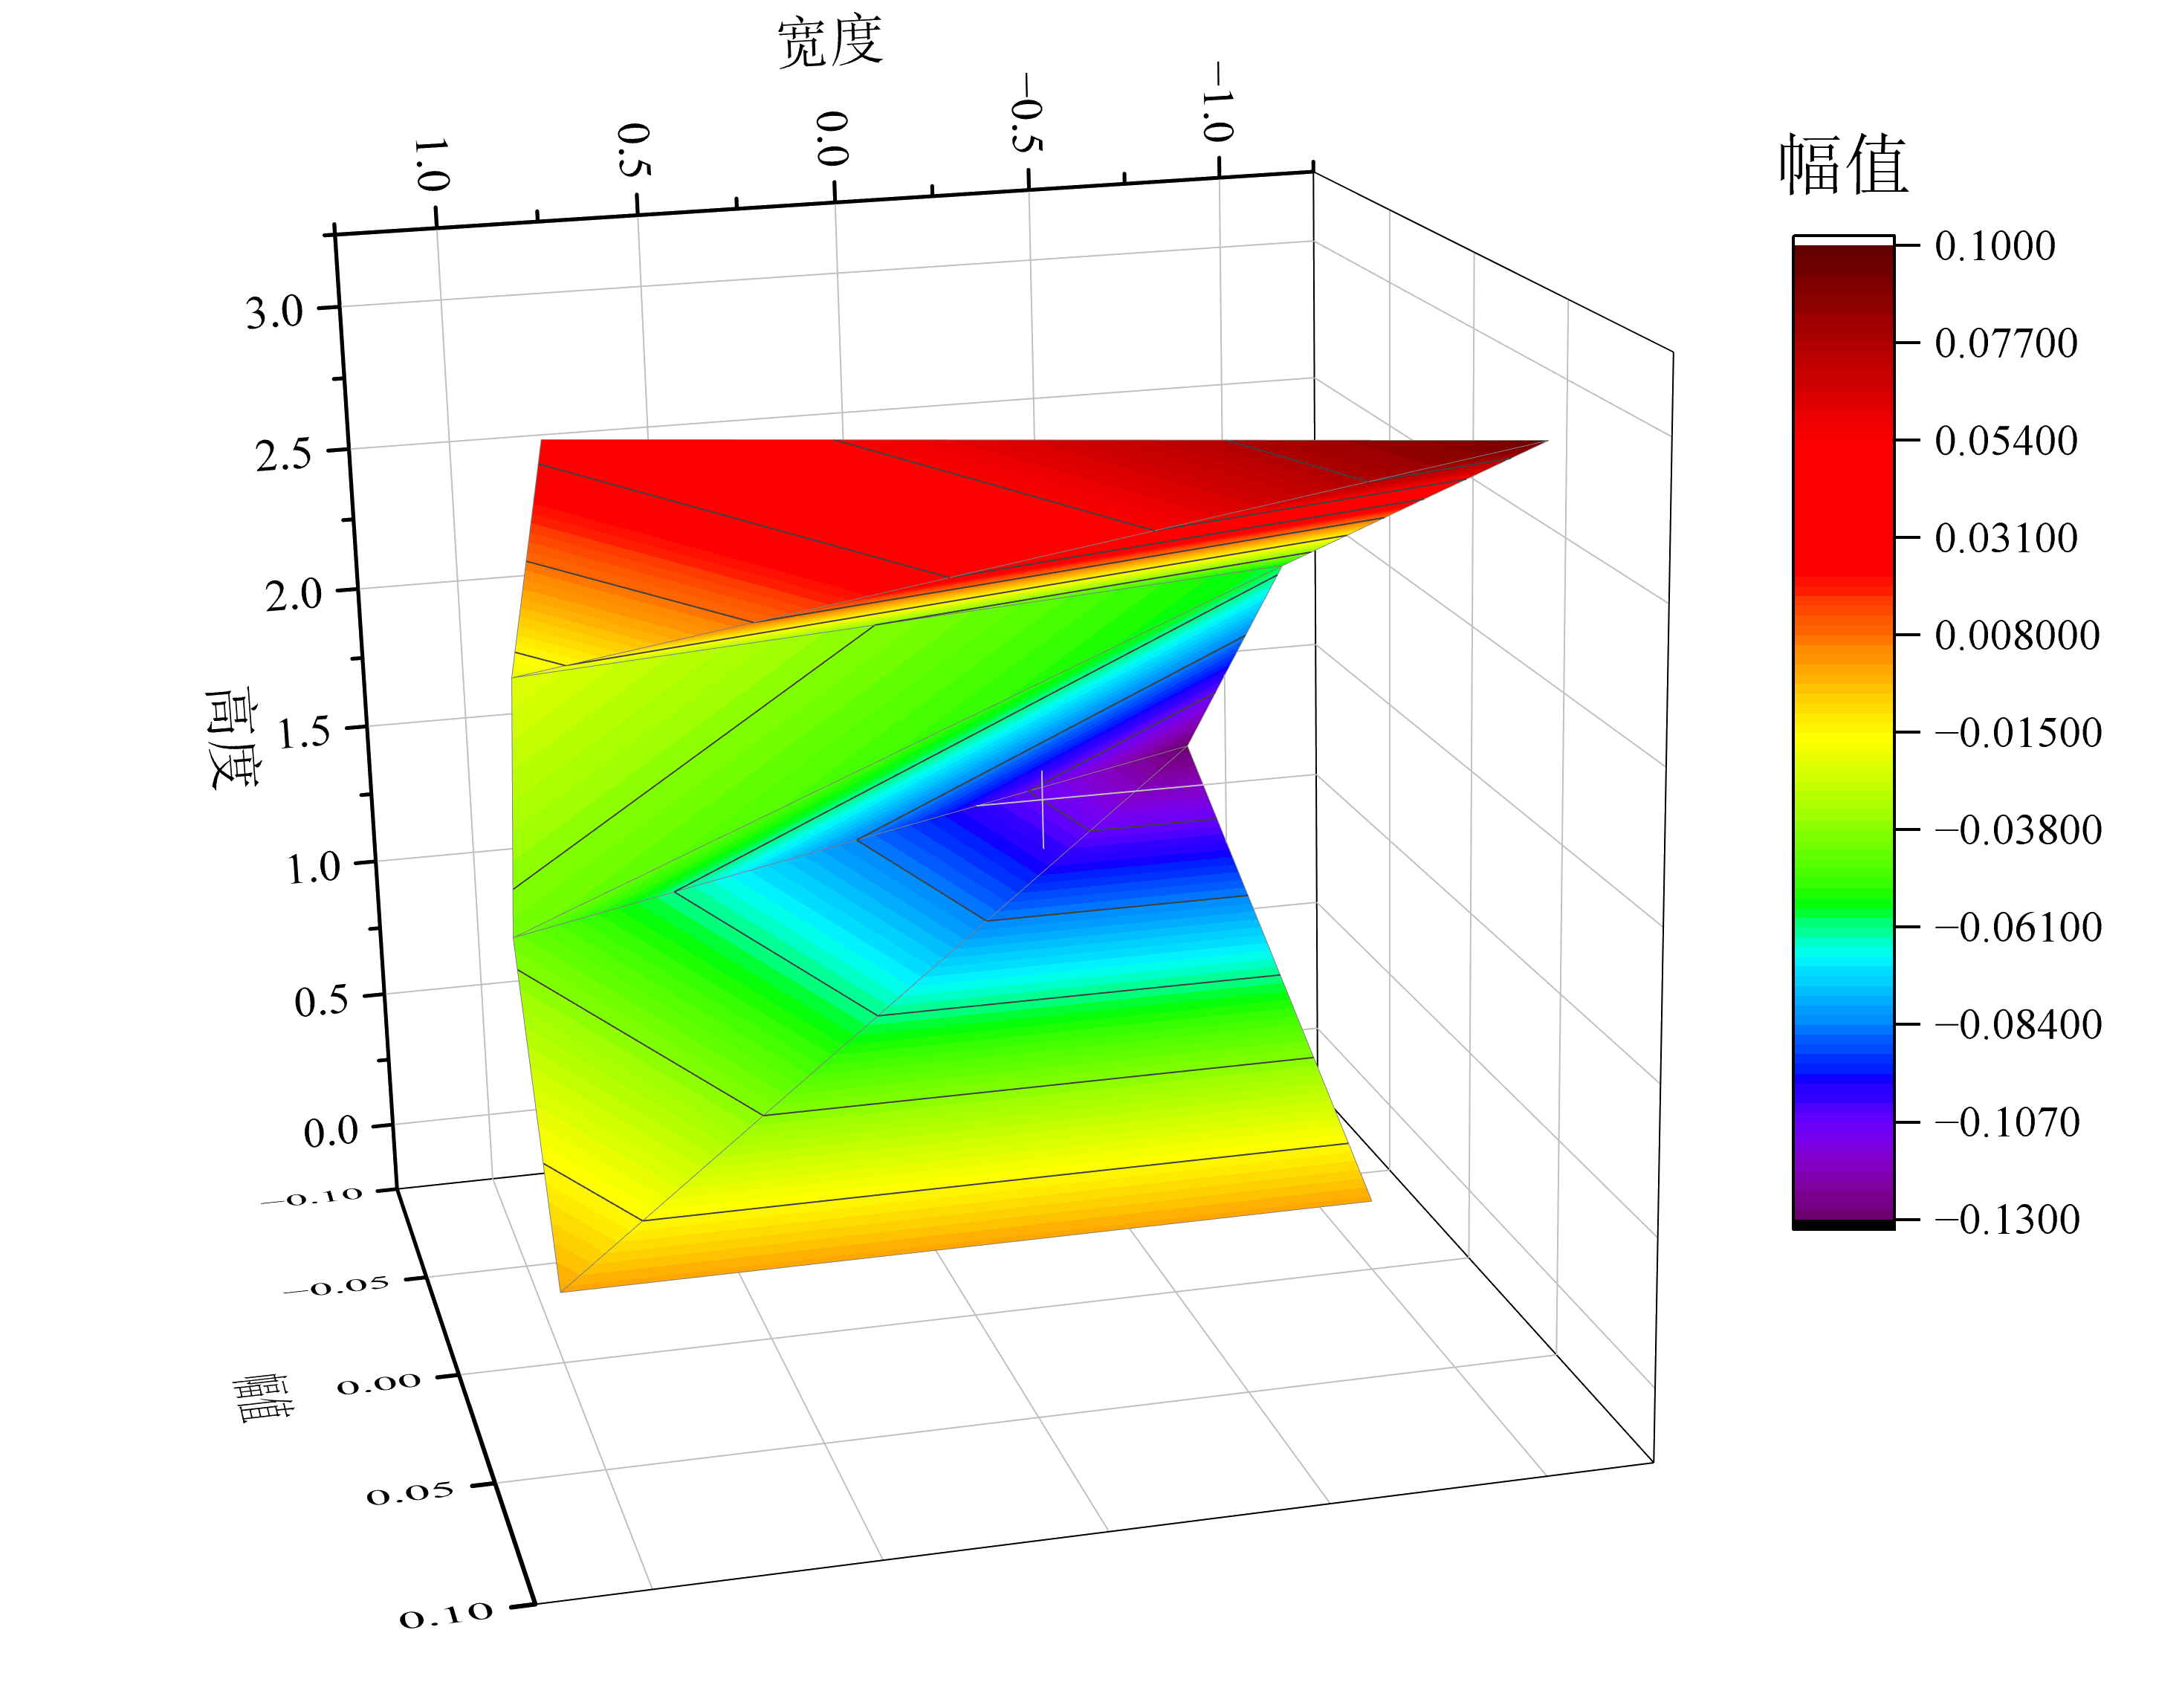
\includegraphics[width=\linewidth]{p17_img03.png}}
\caption{钢锤帽侧面锤击 SISO 振型图（三维图）}
\label{fig:exp4-steel-side-mode3d}
\end{figure}

前三阶固有频率填入表\ref{tab:exp4-steel-side-frequency}，阻尼比填入表\ref{tab:exp4-steel-side-damping}。

\begin{table}[H]
\centering\small
\caption{钢锤帽侧面锤击 SISO 前三阶固有频率}
\label{tab:exp4-steel-side-frequency}
\begin{tabular}{lccc}
\toprule
阶数 & 一阶 & 二阶 & 三阶\\
\midrule
锤击10点（Hz） & \blank[1.5cm] & \blank[1.5cm] & \blank[1.5cm]\\
锤击11点（Hz） & \blank[1.5cm] & \blank[1.5cm] & \blank[1.5cm]\\
锤击12点（Hz） & \blank[1.5cm] & \blank[1.5cm] & \blank[1.5cm]\\
锤击16点（Hz） & \blank[1.5cm] & \blank[1.5cm] & \blank[1.5cm]\\
锤击17点（Hz） & \blank[1.5cm] & \blank[1.5cm] & \blank[1.5cm]\\
锤击18点（Hz） & \blank[1.5cm] & \blank[1.5cm] & \blank[1.5cm]\\
平均（Hz） & \blank[1.5cm] & \blank[1.5cm] & \blank[1.5cm]\\
\bottomrule
\end{tabular}
\end{table}

\begin{table}[H]
\centering\small
\caption{钢锤帽侧面锤击 SISO 阻尼比}
\label{tab:exp4-steel-side-damping}
\begin{tabular}{lccc}
\toprule
阶数 & 一阶 & 二阶 & 三阶\\
\midrule
锤击10点 & \blank[1.5cm] & \blank[1.5cm] & \blank[1.5cm]\\
锤击11点 & \blank[1.5cm] & \blank[1.5cm] & \blank[1.5cm]\\
锤击12点 & \blank[1.5cm] & \blank[1.5cm] & \blank[1.5cm]\\
锤击16点 & \blank[1.5cm] & \blank[1.5cm] & \blank[1.5cm]\\
锤击17点 & \blank[1.5cm] & \blank[1.5cm] & \blank[1.5cm]\\
锤击18点 & \blank[1.5cm] & \blank[1.5cm] & \blank[1.5cm]\\
平均 & \blank[1.5cm] & \blank[1.5cm] & \blank[1.5cm]\\
\bottomrule
\end{tabular}
\end{table}

\section{结果对比、分析与讨论}
\begin{enumerate}
  \item 比较不同锤帽对力锤敲击能量频带的影响：橡胶锤头带宽约为\blank[1.5cm] Hz，尼龙锤头带宽约为\blank[1.5cm] Hz，钢锤头带宽约为\blank[1.5cm] Hz。分析材料硬度、频带宽度及频率分布的关系，并说明测量不同固有频率结构时的锤帽选择原则。
  \item 比较橡胶锤帽 SIMO 与 SISO 两种测量方式得到的振型、固有频率和阻尼比，结果填入表\ref{tab:exp4-compare-simo-siso}。分析两种结果是否一致，以及低频范围内 FFT 数据点稀疏可能造成的读数误差。
\end{enumerate}

\begin{table}[H]
\centering
\caption{橡胶锤帽 SIMO 与 SISO 测得模型弯曲固有频率与阻尼比}
\label{tab:exp4-compare-simo-siso}
\begin{tabular}{lccc}
\toprule
阶数 & 一阶 & 二阶 & 三阶\\
\midrule
SIMO 测得固有频率（Hz） & \blank[1.6cm] & \blank[1.6cm] & \blank[1.6cm]\\
SISO 测得固有频率（Hz） & \blank[1.6cm] & \blank[1.6cm] & \blank[1.6cm]\\
SIMO 测得阻尼比 & \blank[1.6cm] & \blank[1.6cm] & \blank[1.6cm]\\
SISO 测得阻尼比 & \blank[1.6cm] & \blank[1.6cm] & \blank[1.6cm]\\
\bottomrule
\end{tabular}
\end{table}
\answer

比较橡胶锤帽正面敲击和尼龙锤帽侧面敲击的 SISO 结果，填入表\ref{tab:exp4-compare-rubber-nylon}。分析两个方向刚度差异对固有频率和振型的影响。

\begin{table}[H]
\centering
\caption{橡胶锤帽正面敲击与尼龙锤帽侧面敲击结果比较}
\label{tab:exp4-compare-rubber-nylon}
\begin{tabular}{lccc}
\toprule
阶数 & 一阶 & 二阶 & 三阶\\
\midrule
橡胶锤帽正面敲击固有频率（Hz） & \blank[1.4cm] & \blank[1.4cm] & \blank[1.4cm]\\
尼龙锤帽侧面敲击固有频率（Hz） & \blank[1.4cm] & \blank[1.4cm] & \blank[1.4cm]\\
橡胶锤帽正面敲击阻尼比 & \blank[1.4cm] & \blank[1.4cm] & \blank[1.4cm]\\
尼龙锤帽侧面敲击阻尼比 & \blank[1.4cm] & \blank[1.4cm] & \blank[1.4cm]\\
\bottomrule
\end{tabular}
\end{table}
\answer

比较钢锤帽正面和侧面 SISO 测量得到的扭转固有频率、阻尼比与振型，填入表\ref{tab:exp4-compare-steel}。从底座约束、敲击方向、数据读取和振型一致性等方面进行讨论。

\begin{table}[H]
\centering
\caption{钢锤帽正面敲击与侧面敲击结果比较}
\label{tab:exp4-compare-steel}
\begin{tabular}{lccc}
\toprule
阶数 & 一阶 & 二阶 & 三阶\\
\midrule
正面敲击固有频率（Hz） & \blank[1.6cm] & \blank[1.6cm] & \blank[1.6cm]\\
侧面敲击固有频率（Hz） & \blank[1.6cm] & \blank[1.6cm] & \blank[1.6cm]\\
正面敲击阻尼比 & \blank[1.6cm] & \blank[1.6cm] & \blank[1.6cm]\\
侧面敲击阻尼比 & \blank[1.6cm] & \blank[1.6cm] & \blank[1.6cm]\\
\bottomrule
\end{tabular}
\end{table}
\answer

将实验测得的固有频率和固有振型与三自由度系统理论结果进行比较，并讨论阻尼比随模态阶数变化的趋势。
\answer

\section{误差分析}
\begin{enumerate}
  \item 锤击法对实验操作人员要求较高，每次敲击时必须保持力度一致且避免连击。敲击过程中的操作失误可能影响数据的有效性和准确性。
  \item 每次敲击时锤头未必能保证垂直于敲击面，可能导致产生的振动不完全是一维的，进而影响振动模态的准确性。
  \item 每次敲击时，锤击点位置可能无法完全处于结构正中。例如测试弯曲固有频率时，如果锤击点发生偏移，可能同时激发弯曲和扭转振动，进而干扰数据读取。为了避免这一问题，可以使用机械敲击确保锤击点精确定位。
  \item 仪器本身的测量误差可能对结果产生影响，可以通过提高仪器精度减小误差。
  \item 对于低频固有频率的测量，由于采样频率限制，FFT 变换后的数据在低频域内可能较为稀疏，导致难以精确判断频率峰值，从而产生固有频率识别误差。
\end{enumerate}
结合本组曲线和操作过程，补充具体误差来源与改进方法。
\answer

\end{document}
